\documentclass[twoside,a4paper]{article}
% Langage et encodage
\usepackage[english]{babel}
\usepackage[utf8]{inputenc}
\usepackage[T1]{fontenc}
\usepackage{lmodern}

% UPMC recommendations for margin sizes
\usepackage[left=2.5cm,right=2.5cm,top=1.5cm,bottom=2.0cm,includefoot,includehead,headheight=13.6pt]{geometry}
\setlength{\skip\footins}{0.7cm}
\usepackage[bottom]{footmisc}

% Tableaux
\usepackage{longtable}
\usepackage{tabularx}
\usepackage{multirow}
\usepackage{booktabs}
%\addto\captionsfrench{\def\tablename{Table}}

% Typo et formules
\usepackage{eurosym} % Symbole euro
\usepackage{latexsym} % Additional symbols
\usepackage{url} % citer des adresses électroniques et des URL
\usepackage{amsmath,amssymb,amsthm} % AMS Math
\usepackage{leftidx} % Better sub and superscripts
\usepackage[mediumspace,mediumqspace,Grey,squaren]{SIunits} % SI units

% Biblio
\usepackage{natbib} % Package for multiple citation with author-date style
%\setcitestyle{citesep={~;}} % Semicolon separator with french typography
\usepackage{microtype}
\usepackage{breakcites}
\usepackage[hyphenbreaks]{breakurl}
\def\UrlBreaks{\do\/\do-}


% Puces numérotées
\usepackage{enumitem}
\setlist{noitemsep}

% Figures
\usepackage{graphicx}
\usepackage{subfigure}
\usepackage{rotating} % Sideways of figures & tables
\usepackage[singlelinecheck=false]{caption} % Package for caption

%\DeclareCaptionLabelSeparator{virg}{~: } % New caption label separator
%\captionsetup{labelfont=bf,textfont=it,labelsep=virg} % Set fonts and label separators
%\addto\captionsfrench{%
%  \renewcommand{\listfigurename}{Liste des figures}%
%}

%% Table of contents for each chapter
%\usepackage{tocbibind}
%\usepackage[french]{minitoc}
%\setcounter{minitocdepth}{2}
%\mtcindent=15pt
%\renewcommand{\mtcSfont}{\small\normalfont} % Normal font for minitoc entries
%\newcommand{\miniminitoc}{\minitoc \vspace{12pt}}
%% Use \dominitoc at the beginning of the document
%% Use \minitoc where to put a table of contents

% Nicer backref links
\usepackage[breaklinks=true,bookmarks=true,pagebackref,hyperindex=true,pdfa]{hyperref}
\backreffrench
\renewcommand*{\backref}[1]{}
\renewcommand*{\backrefalt}[4]{%
\ifcase #1 %
(Non cited)%
\or
(Cited page~#2)%
\else
(Cited pages~#2)%
\fi}
\renewcommand*{\backrefsep}{, }
\renewcommand*{\backreftwosep}{ and~}
\renewcommand*{\backreflastsep}{ and~}

% Informations included in the pdf file
\hypersetup
{
bookmarksopen=true,
pdftitle="Surface-Wave dispersion Inversion and Profiling",
pdfauthor="Sylvain PASQUET", %auteur du document
pdftoolbar=false, %barre d'outils non visible
pdfmenubar=true, %barre de menu visible
pdfhighlight=/O, %effet d'un clic sur un lien hypertexte
colorlinks=true, %couleurs sur les liens hypertextes
pdfpagemode=UseNone, %aucun mode de page
pdfpagelayout=SinglePage, %ouverture en simple page
pdffitwindow=true, %pages ouvertes entierement dans toute la fenetre
linkcolor=black, %couleur des liens hypertextes internes
citecolor=blue, %couleur des liens pour les citations
urlcolor=black, %couleur des liens pour les url
hyperfootnotes=true
}


\frenchspacing\sloppy
\def\labelitemi{--}
\setlength\parindent{0pt}
\usepackage{parskip}
\parskip=0.75\baselineskip %\advance\parskip by 0pt plus 2pt

\def\SWIP{\textbf{SWIP}}
\def\SU{\textbf{SU}}
\def\SeismicUnix{\textbf{Seismic Unix}}
\def\Geopsy{\textbf{Geospy}}
\def\ImageMagick{\textbf{ImageMagick}}
\def\PDFjam{\textbf{PDFjam}}
\def\pdfcrop{\textbf{pdfcrop}}
\def\MATLAB{\textbf{MATLAB}}
\def\Cygwin{\textbf{Cygwin}}

\title{\Huge{\textbf{SWIP User's Manual}}}
\author{\Large{Sylvain Pasquet} (\url{pasquet.syl@gmail.com})}

\date{\LARGE{Version 1.3: November 2016}\\[2ex]
\large\url{https://github.com/SWIPdev/SWIP/releases}\\
\vspace{2.5cm}
\large{The Surface-Wave dispersion Inversion and Profiling software is supported by:\\
\vspace{1cm}
\textbf{University of Wyoming}\\
Department of Geology and Geophysics\\
Wyoming Center for Environmental Hydrology and Geophysics\\
\bigskip

\includegraphics[scale=0.04]{./figures/logo_UW_brown_2L.png}
\hspace{0.5cm}

\includegraphics[scale=0.05]{./figures/logo_dept_geol_geophy.png}
\hspace{0.5cm}

\includegraphics[scale=0.21]{./figures/logo_WyCEHG.png}\\
\bigskip
Laramie, WY 82070, USA\\
\vspace{1.5cm}
\textbf{Université Pierre et Marie Curie}\\
UMR 7619 METIS\\
\bigskip

\includegraphics[scale=0.095]{./figures/logo_upmc.png}
\hspace{0.5cm}

\includegraphics[scale=0.125]{./figures/logo_metis.png}\\
\bigskip
75005 Paris, France}}


\begin{document}
\maketitle
\thispagestyle{empty}
\newpage
\tableofcontents

\newpage
\section{Quick installation instructions}
If you have experience on how to install and compile codes under a Linux environment, follow these quick installation instructions. More detailed instructions can be found in §\ref{sec:detailedinstruc}.
\begin{enumerate}[leftmargin=*]
\setlength\itemsep{2ex}
\item Install {\MATLAB} (version > 2014a might experience slow figure display and saving).
\item Download {\SWIP} at \url{https://github.com/SWIPdev/SWIP/releases} and add the content of the archive to your {\MATLAB} path.
\item (Windows only) Install {\Cygwin} (32 bits recommended, \url{http://www.cygwin.com/setup-x86.exe}).
\item (Mac OS only) Install \textbf{Xcode}, \textbf{Homebrew} and \textbf{gnu-tar}.
\item Install {\SeismicUnix} (\url{http://www.cwp.mines.edu/cwpcodes}).
\item Install {\Geopsy} (\url{http://www.geopsy.org/download.php}).
\item Install {\SU} extra binaries located in \verb|SWIP/src|.
\item (Optional) Install {\ImageMagick}, {\PDFjam}, and {\pdfcrop}.
\end{enumerate}

\section{How to use SWIP (quick start)}
Here is a quick tutorial to run SWIP and reproduce the figures presented in a paper submitted to Geophysics in December 2016.
\begin{enumerate}[leftmargin=*]
\setlength\itemsep{2ex}
\item In \verb|your_working_directory|, extract the content of the \verb|yellowstone.tar.gz| file located in \verb|SWIP/docs/example|.

\item Download the raw seismic data at \url{http://wycehg.wygisc.org/sharedData/poleMtnGeophysics/Yellowstone/OPTA_072016_1/Seismic.zip} and extract the content of the archive in \verb|your_working_directory/yellowstone|.

\item In {\MATLAB}, go in the extracted folder \verb|your_working_directory/yellowstone| and run the function \verb|seg2su| to create the {\SU} file \verb|swip_profile.su|. Select the \verb|yellowstone/Seismic/Seismic| folder when asked for SEG2 files, then keep a scaling factor of 100 in order to have centimetric precision. Two deployments should be detected, the first one with 2 shots and 240 geophones, the second with 23 shots and 239 geophones (the last trace was killed after the first two shots). Keep this configuration and select the elevation file \verb|OPTA_072016_1_topo.txt| located in the \verb|yellowstone/Seismic| folder. You should obtain a 144.9~Mo file identical to the \verb|swip_profile.su.ok| provided in the archive.

\item Open the script launcher \verb|A_SWIPdisp.m| in {\MATLAB} and run it without changing any parameter (it might take about 45 min to run through the whole line). It will compute dispersion along the acquisition line, with a 31-trace window and shots located on both sides of the window with offset ranging between 0 and 20 traces.It will also resample in wavelength the dispersion curves located in \verb|yellowstone/W31_31.dW1.dS0_20.B/file.pick| and save target files required for the inversion in \verb|yellowstone/W31_31.dW1.dS0_20.B/file.targ|. Finally, it will plot and save 1D data figures (windowed seismogram, corresponding spectrogram, stacked dispersion image with and without picks) in \verb|yellowstone/W31_31.dW1.dS0_20.B/file.img/1D_data|. The 2D pseudo-section of picked phase velocity will also be saved in \verb|yellowstone/W31_31.dW1.dS0_20.B/file.img/|.

\item Run \verb|A_SWIPdisp.m| with \verb|Xmidselec = [16 96]|, \verb|calc = 0|, \verb|plotdisp = 1|, \verb|plotspec = 1|, \verb|plotseismo = 1|, \verb|plotsingle = 1|, \verb|plotstkdisp = 1| (set other plot settings to 0). Select the folder \verb|W31_31.dW1.dS0_20.B| when asked. It will plot individual windowed seismograms along with the corresponding spectrograms and dispersion images for $Xmid = 30$~m and $Xmid = 110$~m. It will also plot intermediate stacked dispersion images.

\item Run \verb|A_SWIPdisp.m| with \verb|calc = 0|, \verb|pick = 1| and \verb|plotpckdisp = 1| to repick and plot dispersion curves.

\item Open the script launcher \verb|B_SWIPparam.m| in {\MATLAB} and run it without changing any parameter. Select the folder \verb|W31_31.dW1.dS0_20.B|, then select the velocity file \verb|yellowstone_vp.txt|. It will then create a semi-automatic parameterization for each $Xmid$ position based on the provided $V_P$ model. These parameterization files, required for the inversion, are stored along with the target files in \verb|yellowstone/W31_31.dW1.dS0_20.B/file.targ|.

\item Open the script launcher \verb|C_SWIPinv.m| in {\MATLAB} and run it without changing any parameter. Select the folder \verb|W31_31.dW1.dS0_20.B| when asked. It will run the inversion for each $Xmid$ position and build a rough pseudo-2D $V_S$ section (the process can take several hours depending on your CPU speed). Inversion results for each $Xmid$ are stored in \verb|yellowstone/W31_31.dW1.dS0_20.B/file.inv/Type1_param|.

\item Run \verb|C_SWIPinv.m| with \verb|Xmidselec = [16 96]|, \verb|inversion = 0| and \verb|plotinvres = 1| to plot inversion results for $Xmid = 30$~m and $Xmid = 110$~m. Select the folder \verb|W31_31.dW1.dS0_20.B|, then the inversion folder \verb|Type1_param|. Resulting figures for the corresponding $Xmid$ will be stored in \verb|yellowstone/W31_31.dW1.dS0_20.B/file.img/Type1_param/models.bweb0/1dmodels|.

\item Open the script launcher \verb|D1_SWIPmod1d.m| in {\MATLAB} and run it without changing any parameter. Select the folder \verb|W31_31.dW1.dS0_20.B|, then the inversion folder \verb|Type1_param|, and finally the velocity file \verb|yellowstone_vp.txt|. It will run the forward modelling for $Xmid = 30$~m and $Xmid = 110$~m and plot final 1D $V_P$, $V_S$, $V_P/V_S$ and Poisson's ratio models. It will also plot theoretical dispersion on top of the dispersion image. Resulting figures for the corresponding $Xmid$ will be stored in \verb|yellowstone/W31_31.dW1.dS0_20.B/file.img/Type1_param/models.bweb0/1dmodels|.

\item Open the script launcher \verb|D2_SWIPmod2d.m| in {\MATLAB} and run it without changing any parameter. Select the folder \verb|W31_31.dW1.dS0_20.B|, then the inversion folder \verb|Type1_param|, and finally the velocity file \verb|yellowstone_vp.txt|. When asksed for an auxiliary data file, select the electrical resistivity file \verb|yellowstone_res.txt|. It will first run the forward modelling along the whole line using $V_P$ from tomography and $V_S$ from SWIP. It will then plot pseudo-2D section of observed and calculated phase velocity along with their residual. It will finally plot final 2D $V_P$, $V_S$, $V_P/V_S$, Poisson's ratio and auxiliary data (i.e. electrical resistivity) models. Resulting figures will be stored in \verb|yellowstone/W31_31.dW1.dS0_20.B/file.img/Type1_param/models.bweb0/2dmodels|, and ASCII \verb|.xzv| files in \verb|yellowstone/W31_31.dW1.dS0_20.B/file.xzv/Type1_param/models.bweb0|

\end{enumerate}

\newpage
\section{Detailed installation instructions}
\label{sec:detailedinstruc}
{\SWIP} is a \MATLAB-based software originally developped to work under a GNU/Linux distribution (but it has been sucessfully installed on Mac OS X and Windows). It executes binaries from the open software packages {\SeismicUnix} and {\Geopsy}. It (optionally) requires the open software packages {\ImageMagick}, {\PDFjam}, and {\pdfcrop}.

Whatever OS you are using, you will need the administrator/root rights to install {\SWIP}.

\subsection{First steps}
Get the latest version of {\SWIP} available at \url{https://github.com/SWIPdev/SWIP/releases}. Download the zipped file \verb|SWIP-x.x.zip| or the gzipped tarfile \verb|SWIP-x.x.tar.gz| containing the source codes for {\SWIP} (the "x.x" is the current release number).

If not already installed, install {\MATLAB} on your computer (no extra toolbox is required). A change of graphics engine in {\MATLAB} 2014b and higher causes problem with figures output (slow figure display, huge output file size). To avoid those problems, I recommend to use an older version of {\MATLAB}.

To download an older version, you need to create a Mathworks account (\url{http://www.mathworks.com}) and download the selected release (\url{http://fr.mathworks.com/downloads/select_release?mode=gwylf}). If you are using a network license, just create an account using your institution email. For a standalone license, you will need to associate it with your Mathworks account in the License Center (\textit{Associate License} on the top right of the screen). When installing {\MATLAB}, you will just need to login to your Mathworks account and provide the path of the license file to activate it.

Once {\MATLAB} is installed, you will need to extract the content of the {\SWIP} archive file in your {\MATLAB} path (refered later as \verb|/your/MATLAB/path|) and give {\MATLAB} access to the contents of this folder. To decompress the gzipped tarfile, use the command \verb|tar -xzf SWIP_xx.tar.gz| in the terminal if you are under Linux or Mac, or use a software like 7zip if you are under Windows. In {\MATLAB}, go in \textit{File->Set Path->Add with Subfolders} to select the \verb|SWIP| folder, then \textit{Save} and \textit{Close}.

Examples of \verb|/your/MATLAB/path| directory:

\verb|/home/yourusername/Documents/MATLAB| under GNU/Linux distributions\\
\verb|/Users/yourusername/Documents/MATLAB| under Mac OS X distributions\\
\verb|C:\Users\yourusername\Documents\MATLAB| under Windows distributions

Type \verb|swip_version| in the MATLAB prompt to check if the scripts are correctly installed.

\clearpage
\subsection{Install on GNU/Linux}
I only tested {\SWIP} with a standard Ubuntu distribution, but the procedure should be similar for other GNU/Linux distributions.
\subsubsection{Prerequisites}
Before installing {\SeismicUnix} and/or {\Geopsy}, you need to make sure that the following libraries and packages are installed on your computer. To install them, type \verb|sudo apt-get install packagename| in the terminal.

\verb|gcc|\\
\verb|gfortran|\\
\verb|qt4-qmake|\\
\verb|libqt4-dev|\\
\verb|liblapack-dev|\\
\verb|libfftw3-dev|\\
\verb|zlib1g-dev|

\subsubsection{Seismic Unix}
\textit{The installation of {\SeismicUnix} ({\SU}) is only necessary to handle seismic data in order to compute, stack and pick dispersion images. If you have your own software for picking dispersion curves and just want to use {\SWIP} to invert them, you can skip the installation of {\SU}.}

The following instructions are mainly copied from the {\SeismicUnix} \verb|Installation_Instructions| file (\url{http://www.cwp.mines.edu/cwpcodes/Installation_Instructions}). Refer to it for more detailed instructions.

Download the latest stable version of {\SU} at \url{http://www.cwp.mines.edu/cwpcodes} (older versions might not be compatible).

Create a directory that will contain all the {\SU} codes (refered later as \verb|/your/SU/path|). This directory should be owned by you (meaning you have write/read/execute rights) and located in a partition with at least 100 Mb available.

Examples of \verb|/your/SU/path| directory:

\verb|/usr/local/SU|\\
\verb|/home/yourusername/SU|\\
\verb|/opt/SU|

Decompress the gzipped tarfile \verb|cwp_su_all_xx.tgz| (the "xx" is the current release number) in \verb|/your/SU/path|, the directory \verb|/your/SU/path/src| will appear, containing all of the source code. To decompress the file, use the command \verb|tar -xzf cwp_su_all_xx.tgz| in the terminal.

In order to set the necessary environment variable and the binaries path, open the file \verb|.profile| located in \verb|/home/yourusername| with a text editor (type \verb|ls -la| in the terminal to see it) and add the following lines at the end of the file:

\verb|export CWPROOT=/your/SU/path|\\
\verb|PATH=$PATH:/your/SU/path/bin|\\
\verb|export PATH|

Run \verb|source .profile| in the terminal and check if these variables are correctly set by typing \verb|echo $CWPROOT| and \verb|echo $PATH|.

In \verb|/your/SU/path/src/configs|, select the file \verb|Makefile.config_your_system| corresponding to your configuration, rename it \verb|Makefile.config| and copy it in \verb|/your/SU/path/src| to replace the existing \verb|Makefile.config|. Then, go in \verb|/your/SU/path/src| by typing \verb|cd /your/SU/path/src| in the terminal. You will then compile the codes by typing:

\verb|make install| => install the basic {\SU} codes\\
\verb|make xtinstall| => install the X windows codes (not necessary for {\SWIP})\\
\verb|make xminstall| => install the Motif based codes (not necessary for {\SWIP})

If you have to recompile along the way, type:

\verb|make remake| => recompile the basic {\SU} codes\\
\verb|make xtinstall| => recompile the X windows based codes (not necessary for {\SWIP})\\
\verb|make xminstall| to recompile the Motif based codes (not necessary for {\SWIP})

Finally, type the command \verb|sukeyword -o| to check if {\SU} is correctly installed.

\subsubsection{SU extra binaries}
Two extra codes, non-available in the default {\SU} release, are required to run {\SWIP}. The first one, \verb|supomegal|, computes the $p-\omega$ transform of a seismogram in the $x-t$ domain in order to retrieve a dispersion image in the $v-f$ domain. The second one, \verb|seg2segy|, allow to convert SEG2 files usually obtained on the field in SEGY files which can then be converted in the {\SU} files required to use {\SWIP} (for more details, see section \ref{sec:seg2su}).

To install these codes, follow these steps in the terminal:

Go in the \verb|SWIP/src| directory by typing: \verb|cd /your/MATLAB/path/SWIP/src|

Assign "execute" permission to the \verb|configure| file by typing: \verb|chmod +x configure|

Compile and install the codes by typing: \verb|./configure|

Type the commands \verb|supomegal| and \verb|seg2segy| in the terminal to check if they are correctly installed.

!! \verb|supomegal| might not compile correctly with older versions of {\SU} (error with \verb|cwp_cexp|) !!

\subsubsection{Geopsy}
For more information about installing {\Geopsy} under Linux, please refer to the {\Geopsy} webpage (\url{http://www.geopsy.org/wiki/index.php/Installation:Linux}).

Download the latest stable Linux version of {\Geopsy} at \url{http://www.geopsy.org/download.php}.

Create a directory that will contain all the {\Geopsy} codes (refered later as \verb|/your/Geopsy/path|). This directory should be owned by you (meaning you have write/read/execute rights) and located in a partition with at least 30 Mb available.\\[1ex]
Examples of \verb|/your/Geopsy/path| directory:

\verb|/usr/local/Geopsy.org| (default)\\
\verb|/home/yourusername/Geopsy.org|\\
\verb|/opt/Geopsy.org|

Decompress the gzipped tarfile \verb|geopsypack-nnitems-src-xx.tgz| ("nn" is the number of items and "xx" is the current release number) in \verb|/your/Geopsy/path|, the directory \verb|/your/SU/path/geopsypack-nnitems-src-xx| will appear, containing all of the source code. To decompress the file, use the command \verb|tar -xzf geopsypack-nnitems-src-xx.tgz| in the terminal.

Set the binaries path in the file \verb|.profile| located in \verb|/home/yourusername| with a text editor (type \verb|ls -la| in the terminal to see it) and extend the \verb|PATH| line (see {\SU} installation) with \verb|:/your/Geopsy/path/bin| such as:

\verb|PATH=$PATH:/your/SU/path/bin:/your/Geopsy/path/bin|

Run \verb|source .profile| in the terminal and check if the path is correctly set by typing \verb|echo $PATH| in the terminal.

In the terminal, go in the \verb|/your/SU/path/geopsypack-nnitems-src-xx| directory by typing \verb|cd /your/SU/path/geopsypack-nnitems-src-xx|.

To configure the installation in the default \verb|/your/Geopsy/path| directory, type:

\verb|./configure|

To configure the installation in a custom \verb|/your/Geopsy/path| directory, type:

\verb|./configure -prefix /your/Geopsy/path|

You will then compile the codes by typing:

\verb|make|\\
\verb|make install|


\subsubsection{Additionnal packages}
Some additionnal packages can be installed to concatenate figure results and produce publication ready final figures (otherwise {\SWIP} produces separate figures). {\ImageMagick} is used to crop and concatenate raster (PNG, JPEG,...) images in order to create figure panels ready for publicactions. {\pdfcrop} cuts the extra edges around PDF created by {\MATLAB}, while {\PDFjam} is used to concatenate PDF images.

Install {\ImageMagick} by typing in the terminal: \verb|sudo apt-get install imagemagick|\\
Install {\PDFjam} by typing in the terminal: \verb|sudo apt-get install pdfjam|\\
Install {\pdfcrop} by typing in the terminal: \verb|sudo apt-get install texlive-extra-utils|

\subsubsection{Known problems}
When starting {\MATLAB} (version < 2011b), the error message \textit{Error while loading shared library libXp.so.6} can appear. A workaround can be found here:

\url{http://fr.mathworks.com/matlabcentral/answers/99815-why-do-i-receive-xsetup-errors-regarding-libxp-so-6-when-installing-or-launching-matlab-on-fedora-co}

When running the inversion (module C, with verbose=1), {\MATLAB} can give you the error message:

\textit{dinver: symbol lookup error: /opt/Geopsy.org/lib/libQGpGuiTools.so.1: undefined symbol: \_ZN12QApplication10commitDataER15QSessionManager}.

It means there is a conflict between Ubuntu QT libraries and {\MATLAB} QT libaries. A workaround is to delete the redundant libraries of {\MATLAB}. These libraries are usually found in:

\verb|/your/MATLAB/path/bin/glnxa64/libQtGui.so.4|\\
\verb|/your/MATLAB/path/bin/glnxa64/libQtNetwork.so.4|\\
\verb|/your/MATLAB/path/bin/glnxa64/libQtCore.so.4|

\clearpage
\subsection{Install on Mac OS X}
{\SWIP} was succesfully installed on El Capitan. It should also work on other versions of Mac OS X.
\subsubsection{Prerequisites}
Before installing {\SeismicUnix} and/or {\Geopsy}, you need to install \textbf{Xcode} which contains the "make" command necessary to compile {\SU} codes. When trying to install {\SU}, it should download it directly, if not, go to \url{https://itunes.apple.com/us/app/xcode/id497799835?mt=12}.

You first need to install \textbf{Homebrew} (\url{http://brew.sh/}) by running this command in the terminal:

\verb|/usr/bin/ruby -e "$(curl -fsSL https://raw.githubusercontent.com/Homebrew/install/master/install)"|

You also need to install \verb|gnu-tar| with:

\verb|brew install coreutils|\\
\verb|brew install gnu-tar|

\subsubsection{Seismic Unix}
\textit{The installation of {\SeismicUnix} ({\SU}) is only necessary to handle seismic data in order to compute, stack and pick dispersion images. If you have your own software for picking dispersion curves and just want to use {\SWIP} to invert them, you can skip the installation of {\SU}.}

The following instructions are mainly copied from the {\SeismicUnix} \verb|Installation_Instructions| file (\url{http://www.cwp.mines.edu/cwpcodes/Installation_Instructions}). Refer to it for more detailed instructions.

Download the latest stable version of {\SU} at \url{http://www.cwp.mines.edu/cwpcodes}

Create a directory that will contain all the {\SU} codes (refered later as \verb|/your/SU/path|). This directory should be owned by you (meaning you have write/read/execute rights) and located in a partition with at least 100 Mb available.

Examples of \verb|/your/SU/path| directory:

\verb|/Users/yourusername/SU|

Decompress the gzipped tarfile \verb|cwp_su_all_xx.tgz| (the "xx" is the current release number) in \verb|/your/SU/path|, the directory \verb|/your/SU/path/src| will appear, containing all of the source code. To decompress the file, use the command \verb|tar -xzf cwp_su_all_xx.tgz| in the terminal.

In order to set the necessary environment variable and the binaries path, open the file \verb|.bash_profile| located in \verb|/Users/yourusername| with a text editor (type \verb|ls -la| in the terminal to see it) and add the following lines at the end of the file (if it doesn't exist, create it by typing \verb|touch .bash_profile|):

\verb|export CWPROOT=/your/SU/path|\\
\verb|PATH=$PATH:/your/SU/path/bin|\\
\verb|export PATH|

Run \verb|source .bash_profile| in the terminal and check if these variables are correctly set by typing \verb|echo $CWPROOT| and \verb|echo $PATH|.

In \verb|/your/SU/path/src/configs|, select the file \verb|Makefile.config_your_system| corresponding to your configuration, rename it \verb|Makefile.config| and copy it in \verb|/your/SU/path/src| to replace the existing \verb|Makefile.config|. Then, go in \verb|/your/SU/path/src| by typing \verb|cd /your/SU/path/src| in the terminal. You will then compile the codes by typing:

\verb|make install| => install the basic {\SU} codes\\
\verb|make xtinstall| => install the X windows codes (not necessary for {\SWIP})\\
\verb|make xminstall| => install the Motif based codes (not necessary for {\SWIP})

If you have to recompile along the way, type:

\verb|make remake| => recompile the basic {\SU} codes\\
\verb|make xtinstall| => recompile the X windows based codes (not necessary for {\SWIP})\\
\verb|make xminstall| to recompile the Motif based codes (not necessary for {\SWIP})

Finally, type the command \verb|sukeyword -o| to check if {\SU} is correctly installed.

\subsubsection{SU extra binaries}
Two extra codes, non-available in the default {\SU} release, are required to run {\SWIP}. The first one, \verb|supomegal|, computes the $p-\omega$ transform of a seismogram in the $x-t$ domain in order to retrieve a dispersion image in the $v-f$ domain. The second one, \verb|seg2segy|, allow to convert SEG2 files usually obtained on the field in SEGY files which can then be converted in the {\SU} files required to use {\SWIP} (for more details, see section \ref{sec:seg2su}).

To install these codes, follow these steps in the terminal:

Go in the \verb|SWIP/src| directory by typing: \verb|cd /your/MATLAB/path/SWIP/src|

Assign "execute" permission to the \verb|configure| file by typing: \verb|chmod +x configure|

Compile and install the codes by typing: \verb|./configure|

Type the commands \verb|supomegal| and \verb|seg2segy| in the terminal to check if they are correctly installed.

!! \verb|supomegal| might not compile correctly with older versions of {\SU} (error with \verb|cwp_cexp|) !!

\subsubsection{Geopsy}
Download the latest stable Mac OS X version of {\Geopsy} at \url{http://www.geopsy.org/download.php} (there is a problem with the El Capitan devel version, so you need to use the sources for Mountain Lion).

Mount the .dmg file, double click and follow the installation instructions. By default, {\Geopsy} will be installed in \verb|/Applications/Geopsy.org| (refered later as \verb|/your/Geopsy/path|).

Set the binaries path in the file \verb|.bash_profile| located in \verb|/Users/yourusername| with a text editor (type \verb|ls -la| in the terminal to see it) and add the following lines at the end of the file:

\verb|PATH=$PATH:/your/Geopsy/path/Utilities|\\
\verb|export PATH|

Run \verb|source .bash_profile| in the terminal and check if the path is correctly set by typing \verb|echo $PATH| in the terminal.

\subsubsection{Additionnal packages}
Some additionnal packages can be installed to concatenate figure results and produce publication ready final figures (otherwise {\SWIP} produces separate figures). {\ImageMagick} is used to crop and concatenate raster (PNG, JPEG,...) images in order to create figure panels ready for publicactions. {\pdfcrop} cuts the extra edges around PDF created by {\MATLAB}, while {\PDFjam} is used to concatenate PDF images.

First of all you need to become the owner of the \verb|/usr/local| directory by running the following command:

\verb|sudo chown -R username /usr/local|

Then to install {\ImageMagick}, run:

\verb|brew link xz libtool jpeg libpng|\\
\verb|brew install imagemagick|

\subsubsection{Known problems}
{\MATLAB}'s bash PATH is different from the Unix PATH, so it will not find the PATH defined in the \verb|.bash_profile| file. A workaround consists in modifying the script that launches {\MATLAB}. Go in the directory where {\MATLAB} is installed (usually \verb|/Applications/MATLAB_R*****.app/bin|). In that folder, you need to open the \verb|matlab| file with a text editor and add the following line after \verb|#!/bin/sh|:

\verb|export PATH:$PATH|

Then you need to make a shortcut of that \verb|matlab| file and run {\MATLAB} with it. If you run your classical {\MATLAB} shortcut, it won't find the correct PATH.

\clearpage
\subsection{Install on Windows}
{\SWIP} has been successfully installed on Windows 7 and Windows 10. The procedure should be very similar on other Windows versions. As mentionned earlier, the Linux-like environment {\Cygwin} is currently required to run {\SeismicUnix} on Windows. However, I don't recommend running {\SWIP} on Windows since the use of a 32 bit version of {\Cygwin} considerably slows down the computation of dispersion images (cf. \ref{sec:cygwin}).

Microsoft has just announced that Windows 10 will soon be able to run Bash and compile Linux binaries with the Windows Subsystem for Linux (\url{https://msdn.microsoft.com/en-us/commandline/wsl/about}). Hopefully we will soon be able to run {\SeismicUnix} without any third party software like {\Cygwin}.

\subsubsection{Cygwin}
\label{sec:cygwin}
Download the 32 bits version of {\Cygwin} available at \url{http://www.cygwin.com/setup-x86.exe} (I could not install {\SU} with the 64 bits version, but if you want to give it a try, be my guest and let me know).

Run \verb|setup-x86.exe|. When asked, choose \textit{Install from Internet}. Select the root directory to install {\Cygwin} (refered later as \verb|\your\cygwin\path|). Make sure it is located in a partition with at least 1 Gb available. Finally, select any of the proposed mirrors to download the data.
Examples of \verb|\your\cygwin\path| directory:

\verb|C:\cygwin| (default)\\
\verb|C:\Program Files\cygwin|

Keep the default install if you don't need {\SU} or {\ImageMagick}. Otherwise add the following packages (use the search bar to find them, then click once on the circle arrow to select them):

\verb|make gcc-core gcc-fortran gcc-g++| in \textit{Devel}\\
\verb|libgcc1 libgfortran3 libmcpp-devel libmcpp0| in \textit{Libs}\\
\verb|ImageMagick| in \textit{Graphics}

Once all the required packages are selected, click Next (keep "select required packages" checked) to start the installation. If you want to use the graphics capabilities of {\SeismicUnix}, you need to install the X11 libraries in {\Cygwin}.

\subsubsection{Seismic Unix}
\label{subsec:WinSU}
\textit{The installation of {\SeismicUnix} ({\SU}) is only necessary to handle seismic data in order to compute, stack and pick dispersion images. If you have your own software for picking dispersion curves and just want to use {\SWIP} to invert them, you can skip the installation of {\SU}.}

The following instructions are mainly copied from the {\SeismicUnix} \verb|Installation_Instructions| file (\url{http://www.cwp.mines.edu/cwpcodes/Installation_Instructions}). Refer to it for more detailed instructions.

Download the latest stable version of {\SU} at \url{http://www.cwp.mines.edu/cwpcodes}

Create a directory that will contain all the {\SU} codes (refered later as \verb|/your/SU/path|). This directory should be owned by you (meaning you have write/read/execute rights) and located in a partition with at least 100 Mb available. I recommend that you create \verb|/your/SU/path| in the root folder of {\Cygwin} \verb|\your\cygwin\path|.

Examples of \verb|/your/SU/path| directory (assuming that you create it from the terminal in the root folder of {\Cygwin}):

\verb|/home/yourusername/SU|\\
\verb|/usr/local/SU|\\
\verb|/opt/SU|

In the Windows Explorer, this directory will look like:

\verb|C:\cygwin\home\yourusername\SU|\\
\verb|C:\cygwin\usr\local\SU|\\
\verb|C:\cygwin\opt\SU|

Decompress the gzipped tarfile \verb|cwp_su_all_xx.tgz| (the "xx" is the current release number) in \verb|/your/SU/path|, the directory \verb|/your/SU/path/src| will appear, containing all of the source code. To decompress the file, use the command \verb|tar -xzf cwp_su_all_xx.tgz| in the {\Cygwin} terminal.

In order to set the necessary environment variable and the binaries path, open the file \verb|.bash_profile| located in \verb|\your\cygwin\path\home\yourusername| with a text editor and add the following lines at the end of the file (!! you need to use the {\Cygwin} path with \verb|/| to define \verb|CWPROOT| and \verb|PATH| in the file !!):

\verb|export CWPROOT=/your/SU/path|\\
\verb|PATH=$PATH:/your/SU/path/bin|\\
\verb|export PATH|

Run \verb|source .bash_profile| in the terminal and check if these variables are correctly set by typing \verb|echo $CWPROOT| and \verb|echo $PATH|.

In the \verb|/your/SU/path/src/configs| directory, select the file \verb|Makefile.config_Cygwin_32|, rename it \verb|Makefile.config| and copy it in \verb|/your/SU/path/src| to replace the existing \verb|Makefile.config|. Then, go in \verb|/your/SU/path/src| by typing \verb|cd /your/SU/path/src| in the terminal. You will compile the codes by typing:

\verb|make install| => install the basic {\SU} codes\\
\verb|make xtinstall| => install the X windows codes (not necessary for {\SWIP})\\
\verb|make xminstall| => install the Motif based codes (not necessary for {\SWIP})

If you have to recompile along the way, type:

\verb|make remake| => recompile the basic {\SU} codes\\
\verb|make xtinstall| => recompile the X windows based codes (not necessary for {\SWIP})\\
\verb|make xminstall| => recompile the Motif based codes (not necessary for {\SWIP})

Finally, type the command \verb|sukeyword -o| to check if {\SU} is correctly installed.

\subsubsection{SU extra binaries}
Two extra codes, non-available in the default {\SU} release, are required to run {\SWIP}. The first one, \verb|supomegal|, computes the $p-\omega$ transform of a seismogram in the $x-t$ domain in order to retrieve a dispersion image in the $v-f$ domain. The second one, \verb|seg2segy|, allow to convert SEG2 files usually obtained on the field in SEGY files which can then be converted in the {\SU} files required to use {\SWIP} (for more details, see section \ref{sec:seg2su}).

To install these codes, follow these steps in the {\Cygwin} terminal:

Go in the \verb|SWIP/src| directory by typing: 

\verb|cd /cygdrive/c/Users/yourusername/Documents/MATLAB/SWIP/src| (if your {\MATLAB} path in Windows is \verb|C:\Users\yourusername\Documents\MATLAB|)

Assign "execute" permission to the \verb|configure| file by typing: \verb|chmod +x configure|

Compile and install the codes by typing: \verb|./configure 32|

Type the commands \verb|supomegal| and \verb|seg2segy| in the terminal to check if they are correctly installed.

!! \verb|supomegal| might not compile correctly with older versions of {\SU} (error with \verb|cwp_cexp|) !!

\subsubsection{Geopsy}
Download the Windows version of {\Geopsy} at \url{http://www.geopsy.org/download.php}.

Execute the file \verb|geopsypack-nnitems-src-xx.exe| ("nn" is the number of items and "xx" is the current release number) and follow the instructions to install {\Geopsy} in \verb|/your/Geopsy/path|.

Example of \verb|/your/Geopsy/path| directory:

\verb|C:\Program Files (x86)\Geopsy.org| (default)

\subsubsection{Setup environment variables}
The final step before using {\SWIP} under Windows is to make sure that the environment variables are correctly set up. The following details correspond to a Windows 7 distribution, it might be slightly different for other versions.

Right click on \textit{Computer -> Properties -> Advanced system settings -> Environment variables}

%% Usefull or not ?
Click on \textit{New} (top one) to create a new User variable:

\textit{Variable name} => \verb|CWPROOT|

\textit{Variable value} => \verb|\your\SU\path|\\
Example => \verb|C:\cygwin\home\yourusername\SU|
%%

Click on \textit{New} (top one) to create a new User variable

\textit{Variable name} => \verb|MATLAB_SHELL|

\textit{Variable value} => \verb|\your\cygwin\path\bin;\your\SU\path\bin;\your\Geopsy\path\bin|\\
Example => \verb|C:\cygwin\bin;C:\cygwin\home\yourusername\SU\bin;C:\Program Files (x86)|

\verb|\Geopsy.org\bin|

Select the system variable \verb|Path| in the bottom list, click on \textit{Edit} (bottom one) and add the following at the end of \textit{Variable value} (the ... correspond to the existing value of the variable):

Variable value => \verb|...;\your\cygwin\path\bin;\your\SU\path\bin;\your\Geopsy\path\bin|\\
Example => \verb|...;C:\cygwin\bin;C:\cygwin\home\yourusername\SU\bin;C:\Program Files (x86)|\\
\verb|\Geopsy.org\bin|

!! Make sure there are no spaces between each path definition !!

Relog your session and check if the environment variables are correctly setup by typing \verb|swip_version| in the {\MATLAB} prompt.

\subsubsection{Additionnal packages}
\label{subsec:WinExtra}
Some additionnal packages can be installed to concatenate figure results and produce publication ready final figures (otherwise {\SWIP} produces separated figures that would need to be concatenated manually).

{\ImageMagick} is used to crop and concatenate raster (PNG, JPEG,...) images in order to create figure panels ready for publicactions. At that point, {\ImageMagick} should have already been installed with {\Cygwin}. However, {\SWIP} uses a function of {\ImageMagick} called \verb|convert| which is redundant with the Windows \verb|convert| function. A workaround consists in creating a link to the {\ImageMagick} \verb|convert| named \verb|img_convert| using the DOS command prompt.

Go in the Windows \textit{Start} menu and search for \textit{cmd} (or go in \textit{Accessories -> Command Prompt})\\
Right click on \textit{cmd} or \textit{Command Prompt} and select \textit{Run as administrator}\\
In the DOS command prompt, type (assuming that the \verb|\your\cygwin\path| directory is \verb|C:\cygwin|):

\verb|mklink "C:\cygwin\bin\img_convert.exe" "C:\cygwin\bin\convert.exe"|

Close the command prompt.

You also need to install \textbf{TeX Live} which contains {\PDFjam} and {\pdfcrop}, two packages required to handle nice PDF figures export. {\pdfcrop} cuts the extra edges around PDF created by {\MATLAB}, while {\PDFjam} is used to concatenate PDF images.

Download the \textbf{TeX Live} Windows installer at \url{http://mirror.ctan.org/systems/texlive/tlnet/install-tl-windows.exe}. Execute the file \verb|install-tl-windows.exe| and select \textit{Custom install}. When asked to select the installation scheme (\textit{Selected scheme} item), choose the option \textit{custom selection of collections}. Then under \textit{Installation collections}, select:

\textit{Essential programs and files}\\
\textit{TeX auxiliary programs}\\
\textit{LaTeX essential packages}\\
\textit{LaTeX supplementary packages}\\
\textit{LaTeX recommended packages}\\
\textit{Windows support programs}

You can also modify the installation directory (refered later as \verb|your\tex\path|) by changing the \textit{TEXDIR (principal TeX directory)} option. Start the installation by clicking on \textit{Install TeX Live}

\subsubsection{Known problems}
\begin{itemize}
\setlength\itemsep{2ex}
\setlength{\parindent}{5ex}
\item {\PDFjam} does not seem to work under Windows, so PDF cannot be concatenated. If you want to create the figure panels, use a raster output format such as PNG or JPEG.

\end{itemize}

\clearpage
\section{How to use {\SWIP} (in details)}

%%%%%
\subsection{Project creation}
\subsubsection{Creating your project directory}
Before starting, you need to create a project directory (referred later as \verb|projdir|) in which seismic data will be processed with {\SWIP}. You need to copy the 5 module launchers of {\SWIP} located in \verb|/your/MATLAB/path/SWIP/launchers| into your project directory.

!! Don't create \verb|projdir| in your {\MATLAB} path !!

!! Don't work in a path containing spaces in one of the folder names !!

\subsubsection{Converting field data in SU format}
\label{sec:seg2su}
Unless you have your own software for picking dispersion curves, you will also need a \verb|.su| file containing all shot gathers in order to compute, stack and pick surface-wave dispersion. The required headers for this \verb|.su| file are \verb|fldr| (field record number), \verb|tracf| (trace number), \verb|gx| (geophone X position), \verb|sx| (source X position), \verb|ns| (number of time samples), \verb|dt| (time sample), \verb|gdel| (mean geophone spacing) and \verb|scalco| (scaling factor, see item list below). You can also add \verb|gelev| (geophone elevation), \verb|selev| (source elevation) to consider the topography. 

For users non familiar with the use of {\SeismicUnix}, the tool \verb|seg2su.m| is provided for an easy creation of \verb|.su| files in \verb|/your/MATLAB/path/SWIP/tools|:

\begin{itemize}[leftmargin=*]
\setlength\itemsep{2ex}
\item Regroup all your SEG2 or SEGY files (e.g. \verb|.dat|, \verb|.sg2|, \verb|.sgy|) in a single folder (referred as \verb|rawdatadir|) located in your \verb|projdir| directory. Individual SEG2 files should be named with increasing numbers (e.g. 1001.dat, 1002.dat,...). If your field data are contained in a single SEGY file, just add this file in the folder instead of the SEG2 files. If you have topography along the line, add a two-column ASCII file (referred as \verb|topofile|) containing the distance and the elevation (X,Z).
\item In {\MATLAB}, go in \verb|projdir| and execute the command \verb|seg2su| in the command window.
\item Select the folder \verb|rawdatadir| when asked for the folder containing SEG2 or SEGY files.
\item Then, define the scaling factor. This factor is used to convert your X and Z coordinates in full integers since {\SU} cannot read decimals. The scaling factor has to be set according to the desired coordinates precision (e.g. a scaling factor of 100 is required if you want a precision of 0.01~m in your geophone X or Z coordinate; coordinates will thus be stored in centimeters).
\item The acquisition setup should then be displayed. Check if the source and geophone positions are correct. When importing SEG2 or SEGY files with non-integer coordinates, only the integer part is read (e.g. 2.5~m becomes 2~m). If that is the case, you need to setup manually the geophones and shots coordinates.
\item When asked, click \textit{No, reset all headers} to manually define the coordinates in the headers. First enter the number of roll-alongs/deployments in the acquisition setup, then for each deployment two vectors [x1 x2 ... xn] of coordinates for the sources and the geophones, respectively.
\item To import topography, click \textit{Yes} when asked, then select the \verb|topofile| in \verb|rawdatadir|. 
\end{itemize}



!! \verb|.su| files created on Windows with {\Cygwin} won't be compatible with other platforms !!

\subsubsection{Importing dispersion curves}
\label{sec:import}
If you have your own software to pick dispersion curves, or if you want to invert dispersion curves picked in a previous project (e.g. to merge dispersion curves obtained from separate profiles), you don't need a \verb|.su| file to use {\SWIP}. In that case, you need to add a folder containing your dispersion curves (3-column ASCII file with frequency, phase velocity and phase velocity error) inside your \verb|projdir| directory. To automatically retrieve the corresponding mode and the position of the dispersion curve along a profile, you can rename your dispersion curves according to the following format: \verb|Xmid.Mmode.pvc|, where \verb|Xmid| is the position along the line and \verb|mode| is the mode number (0 for fundamental, 1 for first higher mode,...). If you want to keep the original file names, you will be able to specify the position and the mode number when importing the dispersion curves (cf \ref{sec:moduleA} - Main settings). You will also need to provide the window size \verb|nW|used to extract dispersion curves and the mean geophone spacing. {\SWIP} will finally create a directory named "W\verb|nW|\_\verb|nW|.dW1.dS1\_1.imported" (hereafter refered as subproject directory or \verb|subprojdir|).

\clearpage
\subsection{SWIP main modules}
For each parameter, you can use the default/automatic settings by commenting the corresponding line in the launcher. {\SWIP} will then read the default setting in the script \verb|SWIP_defaultsettings| located in \verb|/your/MATLAB/path/SWIP/scripts|.


%%%%%
\subsubsection{Module A\_SWIPdisp}
\label{sec:moduleA}
The first module \verb|A_SWIPdisp.m| takes advantage of multi-shot acquisition set-ups to retrieve the lateral variations of surface-wave dispersion using shot gather windowing and dispersion stacking. A range of acceptable window sizes and shot offsets is first defined to extract the data and compute dispersion images using a slant stack in the frequency domain ($p-\omega$ stack). The windows are then shifted along the acquisition profile to obtain a set of dispersion images associated with their corresponding spread mid-point ($Xmid$). Dispersion images associated with an identical $Xmid$ are finally stacked to improve signal-to-noise ratio and enhance the maxima. The shift between two successive extraction windows can range from one receiver spacing to several window lengths. On each stacked dispersion image, the coherent maxima associated with the different propagation modes are identified, picked and extracted with an estimated standard error in phase velocity depending on the frequency and the spread length (the dispersion curves can also be imported from another picking software). The dispersion curves are finally resampled either in wavelength or in frequency, with several criterions limiting their frequency range into reasonable boundaries (e.g. minimum frequency defined according to the spectral amplitude, maximum wavelength defined according to the extraction window length...), and saved in the data format required for the inversion software.

\paragraph{Main settings}
\begin{itemize}[leftmargin=*]
\setlength\itemsep{2ex}
\item \verb|Xmidselec| allows to select all or some of the possible $Xmid$. To select all, keep \verb|Xmidselec| empty or commented. To select one or several $Xmid$, input a list of their number (not position) in the list. The total number of $Xmid$ is contained in the variable \verb|Xlength|, while the $Xmid$ positions are contained in the variable \verb|XmidT|.

\item Set \verb|calc = 1| to compute dispersion images from the \verb|.su| file (cf \ref{sec:seg2su}) or \verb|calc = 2| to import dispersion curves (cf \ref{sec:import}). Once the computation or the importation has been done, you can work with \verb|calc = 0| (for instance to pick/repick dispersion, plot/replot figures, or resample dispersion curves and create inversion target files). When running the code with \verb|calc = 0|, you will be asked to select a subproject directory (cf \ref{sec:moduleA} - Windowing and stacking settings).
\end{itemize}

\paragraph{Windowing and stacking settings (used if calc = 1)}
\begin{itemize}[leftmargin=*]
\setlength\itemsep{2ex}
\item \verb|nWvec| is a vector defining acceptable window sizes (in number of traces) for dispersion computation.

\item \verb|dW| defines the shift (in number of traces) between two successive windows.

\item \verb|dSmin| and \verb|dSmax| define the range of acceptable offsets between the first trace of the window and the shot used to extract the dispersion. For instance, \verb|dSmin = 1| means that the dispersion will start to be extracted from shots located at least one inter-trace spacing away from the first trace, and \verb|dSmax = 5| means that the dispersion will stop being extracted for shots located farther than 5 trace spacings from the first trace.

\item \verb|side| defines if the dispersion is extracted and stacked from shots located on the left ('L'), on the right ('R') or on both sides ('B') of the window.
\end{itemize}

If these parameters are used for the first time, {\SWIP} will create a directory named "W\verb|nWmin|\_\verb|nWmax|.dW\verb|dW|.dS\verb|dSmin|\_\verb|dSmax|.\verb|side|" (hereafter refered as subproject directory or \verb|subprojdir|). If the subproject directory already exists, {\SWIP} will overwrite the existing data for the selected $Xmid$. The data  are stored in the \verb|file.dat| folder, created in \verb|projdir/subprojdir|. It contains 3 different {\SU} files for each $Xmid$ position (example of windowed seismogram \verb|Xmid.sum.su|, spectrogram of the example of windowed seismogram \verb|Xmid.sum.spec| and stacked dispersion image \verb|Xmid.sum.dsp|). It also contains a \verb|project.param.mat| file with the main subproject parameters (!! do not delete that file !!).

\begin{figure}[h!]
\centerline{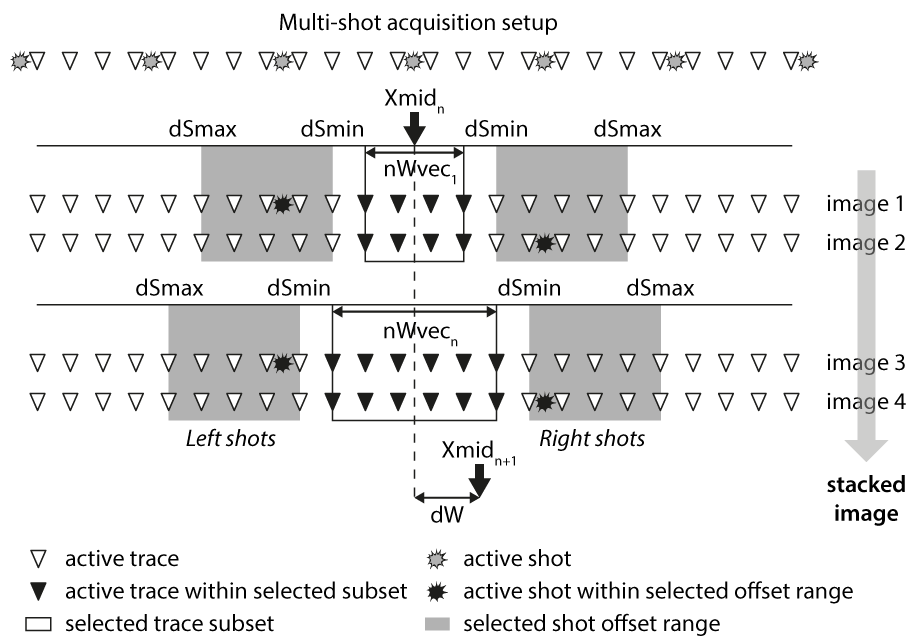
\includegraphics[width=0.75\linewidth]{figures/stack_wind.png}}
\caption{Stacking and windowing workflow. (1) select seismic data subsets centered on a specific position ($Xmid$) with window sizes defined by the vector $nWvec$ containing the number of traces of each window; (2) select shots illuminating the selected subsets with offsets ranging between $dSmin$ and $dSmax$ traces on both side of each subset; (3) extract the selected subsets from the shot records for each pair of shot and window size; (4) transform the wavefield to the frequency-phase velocity domain (dispersion image) for each selected subsets; (5) normalize amplitude spectrum at each frequency for each dispersion image; (6) stack all normalized dispersion images computed at the same $Xmid$; (7) shift the window of $dW$ traces and repeat steps 1-6 to the next $Xmid$.}
\label{fig:stack_wind}
\end{figure}

\paragraph{P-omega transform settings (used if calc = 1)}
\begin{itemize}[leftmargin=*]
\setlength\itemsep{2ex}
\item \verb|fmin| and \verb|fmax| define the frequency range (in Hz) for dispersion image computation ($p-\omega$ stack).

\item \verb|nray| defines the number of phase velocity samples for the $p-\omega$ stack.

\item \verb|vmin| and \verb|vmax| define the range of phase velocity (in m/s) for the $p-\omega$ stack.
\end{itemize}

\paragraph{Filter and mute settings (used if calc = 1)}
\begin{itemize}[leftmargin=*]
\setlength\itemsep{2ex}
\item Set \verb|filt = 1| to apply a band pass filter to the seismic data before the $p-\omega$ stack, or \verb|filt = 0| otherwise.

\item \verb|fcutlow| and \verb|fcuthigh| define the frequency limits of the filter (in Hz).

\item \verb|taper| defines the width of the taper window (in Hz).

\item Set \verb|mute = 1| to apply a mute\footnote{The mute consists in zeroing samples before and/or after a specific time.} to the seismic data before the $p-\omega$ stack, or \verb|mute = 0| otherwise. The mute is applied to each windowed seismogram, and is linear between the shortest offset trace (trace 1) and the largest offset trace (trace 2)

\item \verb|tmin1| and \verb|tmin2| define the first and last trace upper mute limits (in s).

\item \verb|tmax1| and \verb|tmax2| define the first and last trace lower mute limits (in s).
\end{itemize}

\paragraph{Dispersion picking settings}
\begin{itemize}[leftmargin=*]
\setlength\itemsep{2ex}
\item Set \verb|pick = 1| to manually pick dispersion curves. I recommend to first start the script with \verb|calc = 1| and \verb|pick = 0|, then once it's done computing dispersion images, restart the script with \verb|calc = 0| and \verb|pick = 1| (picking while calculating can take a long time). To use the automatic picking option (\verb|pick = 2|), you first need to pick one dispersion curve with \verb|pick = 1|. It will then look for dispersion maxima in the range of the first picked dispersion curve (this option is still experimental).

\item \verb|mappick| defines the colormap used for the picking. While picking, you will be able to change the colormap for a specific $Xmid$, but it will reset to \verb|mappick| for each new $Xmid$.

\item Set \verb|mappicklog = 1| to use a "pseudo-logarithmic" colorscale to enhance mode identification, or \verb|mappicklog = 0| for a linear colorscale.

\item \verb|dvmin| defines the minimum phase velocity sample (in m/s) used to display and pick the dispersion. This option is used to speed up display when picking, but will reduce the resolution of the picked phase velocity dispersion curves, which can be critical when dealing with small velocity variations.

\item \verb|modeinit| defines the first mode that is picked (0 corresponding to the fundamental mode, 1 to the first higher mode,...). While picking, you will be able to change the picked mode for a specific $Xmid$, but it will reset to \verb|modeinit| for each new $Xmid$.

\item Set \verb|pickstyle = 1| to use semi-automatic picking (finds the closest maxima around the pick), or \verb|pickstyle = 0| to use full manual picking. While picking, you will be able to change the picking style for a specific $Xmid$, but it will reset to \verb|pickstyle| for each new $Xmid$.

\item Set \verb|smoothpick = 1| to smooth the picks with a moving average filter, or \verb|smoothpick = 0| for no smoothing. While picking, you will be able to change the smoothing style for a specific $Xmid$, but it will reset to \verb|smoothpick| for each new $Xmid$.
\end{itemize}

Picked dispersion curves are stored in \verb|subprojdir/file.pick|. They are named according to the $Xmid$ position and the corresponding mode (\verb|Xmid.Mmode.pvc|), and contain three columns with the frequency, phase velocity and phase velocity error.

Several options are available during picking:
\begin{itemize}[leftmargin=*]
\item \verb|ENTER| or close picking window: Save current picks and go to next $Xmid$
\item \verb|BACKSPACE|: Save current picks and go to previous $Xmid$
\item \verb|H|: Save current picks and go to next (higher) mode
\item \verb|L|: Save current picks and go to previous (lower) mode
\item \verb|W|: Save current picks and stop script
\item \verb|A|: Discard current picks and go to next $Xmid$  (keep previous picks)
\item \verb|Z|: Discard current picks and go to previous $Xmid$ (keep previous picks)
\item \verb|N|: Discard current picks and go to next (higher) mode (keep previous picks)
\item \verb|P|: Discard current picks and go to previous (lower) mode (keep previous picks)
\item \verb|X|: Discard current picks and stop script (keep previous picks)
\item \verb|M|: Switch between manual and semi-automatic picking
\item \verb|S|: Switch between smooth and regular picking
\item \verb|D|: Delete one or several points (keep the mouse button pushed while moving the pointer to delete points, then press ENTER to resume picking).
\item \verb|R|: Reset all picks
\item \verb|E|: Change error style (no error, percentage or lorentz)
\item \verb|C|: Open colormap editor
\end{itemize}

If the picking freezes, close the window to go to the next $Xmid$ (this will save the current picks).

\paragraph{Dispersion curves sampling settings}
\begin{itemize}[leftmargin=*]
\setlength\itemsep{2ex}
\item Set \verb|target = 1| to convert picked dispersion curves into the target files required for the inversion software, or \verb|target = 0| otherwise.

\item Set \verb|wave = 'R'| to create Rayleigh waves target, or \verb|wave = 'L'| to create Love waves target.

\item \verb|maxmodeinv| defines the maximum number of mode included in the target file (and that will be inverted). Leave empty to include all the picked modes (up to 10 by default).

\item Set \verb|sampling = 1| to resample the picked dispersion curves in wavelength, or \verb|sampling = 0| to resample the picked dispersion curves in frequency. A discretization in wavelength is generally recommended to invert depth consistent data and prevent from giving excessive weight to high frequency samples which correspond only to the shallowest part of the medium.

\item \verb|resampvec| defines the vector along which dispersion curves are resampled. It has to be a wavelength vector (in m) if \verb|sampling = 1|, and a frequency vector (in Hz) if \verb|sampling = 0|.\\[1ex]
!! This vector is critical since it will limit the range of the dispersion saved in the target file. Even if you pick dispersion curves down to a given frequency, the range of \verb|resampvec| (especially when you resample in wavelength) can prevent the target dispersion curves to reach that frequency. This is clear when comparing the picked dispersion image saved in \verb|subprojdir/file.img/1D_data/disp_pick| with the picked dispersion image displayed during picking. !!

\item Set \verb|freqlim = 0| to set manually the minimum frequency of the resampled dispersion curve, or \verb|freqlim = 1| to use an automatic cutoff frequency determined from an amplitude threshold on the spectrogram (cf. \verb|specampmin|).\\[1ex]
!! By default, this cutoff frequency is displayed as a dashed red line during picking !!

\item \verb|specampmin| is the minimum amplitude of the spectrogram (in normalized units) used to determine the automatic cutoff frequency.\\[1ex]
\end{itemize}

Target files are stored in \verb|subprojdir/file.targ| and contain all modes selected for inversion (cf option \verb|maxmodeinv|). They are named according to their $Xmid$ position (\verb|Xmid.target|). If a target file already exists for the selected $Xmid$ when using \verb|target = 1|, it will be overwritten. Run the script with \verb|calc = 0| and \verb|pick = 0| to change only the targets parameter (sampling, number of included modes, error type,...).

\paragraph{Error settings (used if target = 1)}
\begin{itemize}[leftmargin=*]
\setlength\itemsep{2ex}
\item Set \verb|err = 1| to define an empirical phase velocity error depending on the frequency and the window size (Lorentz error), \verb|err = 2| to define a percentage phase velocity error, or \verb|err = 0| for no error.

\item \verb|nWfac| allows to tweak the Lorentz error in order to increase (\verb|nWfac < 1|) or reduce (\verb|nWfac > 1|) the size of the error bars by calculating the error as if the mean window size $nW$ was actually $nW*nWfac$. It is used only if \verb|err = 1|.

\item \verb|minerrvel| is the minimum velocity error (in m/s) allowed when \verb|err = 1|. It prevents from having too small error bars at high frequency in which no theoretical model could fit.

\item \verb|maxerrrat| is the maximum velocity error ratio allowed when \verb|err = 1|. It prevents from having too large error bars at low frequency in which all theoretical models could fit.

\item \verb|sigma| is the percentage of the velocity used to define the error when \verb|err = 2|.
\end{itemize}

\paragraph{Plot settings}
\begin{itemize}[leftmargin=*]
\setlength\itemsep{2ex}
\item Set \verb|plotdisp = 1| to plot and save dispersion images in \verb|subprojdir/file.img/1D_data/disp| (\verb|plotdisp = 0| for no plot).

\item Set \verb|plotpckdisp = 1| to plot and save stacked dispersion images with picked dispersion curves in \verb|subprojdir/file.img/1D_data/disp_pick| (\verb|plotpckdisp = 0| for no plot).

\item Set \verb|plotspec = 1| to plot and save spectrograms in \verb|subprojdir/file.img/1D_data/spectro| (\verb|plotspec = 0| for no plot).

\item Set \verb|plotseismo = 1| to plot and save seismograms in \verb|subprojdir/file.img/1D_data/seismo| (\verb|plotseismo = 0| for no plot).

\item Set \verb|plotsingle = 1| to plot and save prestack single seismogram (if \verb|plotseismo = 1|), spectrograms (if \verb|plotspec = 1|) and dispersion images (if \verb|plotdisp = 1|) in \verb|subprojdir/file.img/1D_data/prestack/Xmid_xmid| (\verb|plotsingle = 0| for no plot).

\item Set \verb|plotstkdisp = 1| to plot and save intermediate stacked dispersion images in \verb|subprojdir/file.img/1D_data/synstack/Xmid_xmid| (\verb|plotstkdisp = 0| for no plot).

\item Set \verb|plot1dobs = 1| to plot and save dispersion curves in \verb|subprojdir/file.img| (\verb|plot1dobs = 0| for no plot).

\item Set \verb|plot2dobs = 1| to plot and save phase velocity pseudo-section in \verb|subprojdir/file.img| (\verb|plot2dobs = 0| for no plot).

\item Set \verb|showplot = 1| to display the plots on the screen (\verb|showplot = 0| for no display).
\end{itemize}

\paragraph{Figure display and output settings}
\begin{itemize}[leftmargin=*]
\setlength\itemsep{2ex}
\item \verb|imgform| defines the output format of figures. It can be \verb|'PDF'|, \verb|'PNG'|, \verb|'JPEG'|, \verb|'TIFF'| or \verb|'FIG'|.

\item \verb|imgres| defines the resolution of raster figures in DPI (dot per inch).

\item \verb|fs| defines the font size of the figures.

\item \verb|cbpos| defines the position of colorbars (=1, colorbar on the right; =2, colorbar at the bottom).
\end{itemize}

\paragraph{Dispersion, spectrograms and seismograms settings}
\begin{itemize}[leftmargin=*]
\setlength\itemsep{2ex}
\item Set \verb|Dlogscale = 1| to use a "pseudo-logarithmic" colorscale in the saved dispersion images (\verb|Dlogscale = 0| for linear colorscale).

\item Set \verb|Flogscale = 1| to use a logarithmic frequency axis in the saved dispersion images and dispersion curves (\verb|Flogscale = 0| for linear axis).

\item Set \verb|axetop = 1| to display the X axis at the top of saved dispersion images, spectrograms and dispersion curves (\verb|axetop = 0| for X axis at the bottom).

\item Set \verb|axerev = 1| to display the Y axis pointing downward in the saved dispersion images, spectrograms and dispersion curves (\verb|axetop = 0| for Y axis pointing upward).

\item Set \verb|cb_disp = 1| to display colorbar on dispersion images and spectrograms (\verb|cb_disp = 0| for no colorbar).

\item Set \verb|plotflim = 1| to plot the low frequency cut defined with \verb|freqlim| (cf \ref{sec:moduleA} - Dispersion curves sampling settings). (\verb|plotflim = 0| for no plot).

\item Set \verb|plotlamlim = 1| to plot the maximum wavelength defined by \verb|resampvec| (cf \ref{sec:moduleA} - Dispersion curves sampling settings). (\verb|plotlamlim = 0| for no plot).

\item Set \verb|eb = 1| to display errorbars on dispersion curves when \verb|plotpckdisp = 1| or \verb|plot1dobs = 1| (\verb|eb = 0| for no errorbars).

\item \verb|pickcol1| and \verb|pickcol2| define the color of even and odd mode numbers, respectively, plotted on dispersion images when \verb|plotpckdisp = 1| (e.g. \verb|'w'| for white, \verb|'r'| for red, \verb|'k'| for black, \verb|'b'| for blue).\\[2ex]

\item \verb|map0| defines the colormap for dispersion images and spectrograms.

\item \verb|fMIN|, \verb|fMAX| and \verb|fticks| control the display of frequency limits and ticks on dispersion images, spectrograms and dispersion curves (in Hz).

\item \verb|VphMIN|, \verb|VphMAX| and \verb|Vphticks| control the display of phase velocity limits and ticks on dispersion images (in m/s).

\item \verb|tMIN|, \verb|tMAX| and \verb|tticks| control the display of time limits and ticks on seismograms (in ms).
\end{itemize}

\paragraph{Phase velocity pseudo-section settings}
\begin{itemize}[leftmargin=*]
\setlength\itemsep{2ex}
\item \verb|map1| defines the colormap for picked phase velocity pseudo-sections.

\item \verb|xMIN|, \verb|xMAX| and \verb|xticks| control the display of X limits and ticks on the pseudo-section (in m).

\item \verb|lamMIN|, \verb|lamMAX| and \verb|lticks| control the display of wavelength limits and ticks on the pseudo-section (in m).

\item \verb|vphMIN|, \verb|vphMAX| and \verb|vphticks| control the display of phase velocity limits and ticks on the pseudo-section (in m/s).
\end{itemize}


%%%%%
\subsubsection{Module B\_SWIPparam}
The second module \verb|B_SWIPparam.m| allows to build a parameterization used in the inversion. It can either create a completely user-defined parameterization, or different possibility of semi-automatic parameterization based on P-wave traveltime tomography results.

\paragraph{Main settings}
\begin{itemize}[leftmargin=*]
\setlength\itemsep{2ex}
\item \verb|Xmidselec| allows to select all or some of the possible $Xmid$. To select all, keep \verb|Xmidselec| empty or commented. To select one or several $Xmid$, input a list of their number (not position) in the list. The total number of $Xmid$ is contained in the variable \verb|Xlength|, while the $Xmid$ positions are contained in the \verb|XmidT| variable.

\item Set \verb|paramname = []| to use a default name based on the parameters. You can also set a specific name (e.g. \verb|paramname = 'myparametername'|).

\item Set \verb|paramtype = 0| to create an arbitrary parameterization based only on the user input. This \verb|.param| file will be stored in \verb|projdir/file.param|.\\[1ex]
Set \verb|paramtype = 1| to create a parameterization with varying thicknesses and a reduced range of $V_P$ defined from a P-wave tomography model.\\[1ex]
Set \verb|paramtype = 2| to create a parameterization with varying thicknesses and a fixed $V_P$ defined from a P-wave tomography model.\\[1ex]
Set \verb|paramtype = 3| to create a parameterization with fixed thicknesses and a reduced range of $V_P$ defined from a P-wave tomography model.\\[1ex]
Set \verb|paramtype = 4| to create a parameterization with fixed thicknesses and fixed $V_P$ defined from a P-wave tomography model.\\[1ex]
For \verb|paramtype > 0|, a specific \verb|Xmid.param| file will be stored for each $Xmid$ along with the \verb|Xmid.target| files in the \verb|subprojdir/file.targ| directory. The input of a three column ($X,Z,V_P$) ASCII file is required (if using Excel for Mac OS, you need to save the velocity model as a \textit{Windows Formatted Text} file).
\end{itemize}

\paragraph{Parameter space settings}
\begin{itemize}[leftmargin=*]
\setlength\itemsep{2ex}
\item \verb|nlay| controls the number of layers (including half-space) of the parameter space.\\[1ex]

The following settings can be either scalars (same parameters for all layers) or vectors with \verb|nlay| elements (specific parameters for each layer).\\
\item \verb|nsublay| controls the number of sublayers in each layer (used if \verb|shape>1|).

\item \verb|thmin| defines the minimum thickness of each layer (in m).

\item \verb|thmax| defines the maximum thickness of each layer (in m).\\[2ex]

\item Set \verb|lvz = 1| to allow lower velocity than in the previous layer (or \verb|lvz = 0| to prevent it).

\item Set \verb|shape = 1| to use a uniform velocity for each layer.\\[1ex]
Set \verb|shape = 2| to force a linear variation with depth.\\[1ex]
Set \verb|shape = 3| to force a linear increase with depth.\\[1ex]
Set \verb|shape = 4| to force a linear decrease with depth.\\[1ex]
Set \verb|shape = 5| force a power law increase with depth.\\[2ex]

\item \verb|Vsmin| defines the minimum shear-wave velocity of each layer (in m/s).

\item \verb|Vsmax| defines the maximum shear-wave velocity of each layer (in m/s).

\item \verb|Vpmin| defines the minimum pressure-wave velocity of each layer (in m/s).

\item \verb|Vpmax| defines the maximum pressure-wave velocity of each layer (in m/s).

\item \verb|Rhomin| defines the minimum density of each layer (in kg/m$^3$).

\item \verb|Rhomax| defines the maximum density of each layer (in kg/m$^3$).

\item \verb|Numin| defines the minimum Poisson's ratio of each layer.

\item \verb|Numax| defines the maximum Poisson's ratio of each layer.\\[2ex]

\item Set \verb|Vplink = 1| to link the $V_P$ thickness with the $V_S$ thickness (recommended), or \verb|Vplink = 0| to invert for separate thicknesses.

\item Set \verb|Rholink = 1| to link the density thickness with the $V_S$ thickness (recommended), or \verb|Rholink = 0| to invert for separate thicknesses.

\item Set \verb|Nulink = 1| to link the Poisson's ratio thickness with the $V_S$ thickness (recommended), or \verb|Nulink = 0| to invert for separate thicknesses.
\end{itemize}

\paragraph{Semi-automatic parameterization settings (used if paramtype $\neq$ 0)}
\begin{itemize}[leftmargin=*]
\setlength\itemsep{2ex}
\item Set \verb|plot2dVP = 1| to display the imported $V_P$ model (or \verb|plot2dVP = 0| for no plot).

\item \verb|dz| controls the sampling in depth of the imported $V_P$ model (in m).

\item \verb|vfac| controls the range of $V_P$ (\verb|Vpmin-vfac*Vpmin<Vp<Vpmax+vfac*Vpmax|)

\end{itemize}

\subsubsection{Module C\_SWIPinv}
\label{sec:moduleC}
The third module \verb|C_SWIPinv.m| allows to perform the Monte Carlo inversion for each $Xmid$ using the Neighborhood Algorithm (NA). For each inversion, several options are proposed to build the final 1D $V_S$ model: (i) using the model with the lowest misfit; (ii) using an average of the n models with the lowest misfits; (iii) or using an average of all models whose calculated dispersion curves fit the observed data within the error bars. In the two latter cases, the final average model can be constructed either by taking the actual mean value of each parameter, or by weighting the different parameters according to each model’s misfit.

\paragraph{Main settings}
\begin{itemize}[leftmargin=*]
\setlength\itemsep{2ex}
\item \verb|Xmidselec| allows to select all or some of the possible $Xmid$. To select all, keep \verb|Xmidselec| empty or commented. To select one or several $Xmid$, input a list of their number (not position) in the list. The total number of $Xmid$ is contained in the variable \verb|Xlength|, while the $Xmid$ positions are contained in the \verb|XmidT| variable.

\item Set \verb|inversion = 1| to run the inversion (or \verb|inversion = 0| to use existing inversion results, for instance to replot or recalculate average model with different settings).

\end{itemize}

\paragraph{Inversion settings (used if inversion = 1)}
\begin{itemize}[leftmargin=*]
\setlength\itemsep{2ex}
\item Set \verb|paramtype = 0| to use an arbitrary parameterization based only on the user input. It will ask to input a \verb|.param| file stored in \verb|projdir/file.param|.\\[1ex]
Set \verb|paramtype = 1| to use a parameterization with varying thicknesses and a reduced range of $V_P$ defined from a P-wave tomography model.\\[1ex]
Set \verb|paramtype = 2| to use a parameterization with varying thicknesses and a fixed $V_P$ defined from a P-wave tomography model.\\[1ex]
Set \verb|paramtype = 3| to use a parameterization with fixed thicknesses and a reduced range of $V_P$ defined from a P-wave tomography model.\\[1ex]
Set \verb|paramtype = 4| to use a parameterization with fixed thicknesses and fixed $V_P$ defined from a P-wave tomography model.

\item \verb|nrun| defines the number of run in the NA inversion process.

\item \verb|itmax| defines the number of iterations per run.

\item \verb|ns0| defines the number of models generated at the beginning of each run.

\item \verb|ns| defines the number of models generated at each iteration of each run.

\item \verb|nr| defines the number of previously generated models used to build a new sub-parameter space in which models will be generated at the next iteration.

\item Set \verb|verbose = 1| to display NA inversion process information (\verb|verbose = 0| for no display). Setting \verb|verbose = 0| considerably speed up the inversion process. If \verb|verbose = 0| and the inversion display remains on "Run 1", restart the inversion with \verb|verbose = 1| to figure out the problem.
\end{itemize}

For each inversion run, the parameter space is divided in \verb|ns0| Voronoi cells centered on each generated model, with boundaries in each parameter direction being equidistant from the nearest neighbour model. The \verb|nr| best cells (i.e. with the lowest misfit) are then selected, within which \verb|ns/nr| new models are randomly generated. The \verb|ns| new models are finally added to the previous ones, updating the Voronoi cell distribution. This operation is repeated for \verb|itmax| iterations until reaching \verb|ns0 + ns * itmax| generated models.

Inversion results are stored in \verb|subprojdir/file.inv/inv_paramname_or_type/Xmid_reports| in gzipped files \verb|run_##.report.gz| along with the corresponding target file \verb|Xmid.target| and parameterization file (this prevents from losing the inverted data when modifying picks and/or sampling of targets in module A).

\paragraph{Average models calculation settings}
\begin{itemize}[leftmargin=*]
\setlength\itemsep{2ex}
\item Set \verb|nbest = 0| to extract best models fitting the error bars, or set \verb|nbest > 0| to extract the best \verb|nbest| models (based on the misfit value).

\item \verb|outpoints| defines the number of data samples that are allowed to be out of the error bars when using \verb|nbest = 0|.

\item \verb|dz| controls the sampling in depth of the smooth $V_S$ model (in m).
\end{itemize}

!! If none or only a few of the generated models fit within the error bars when running the code with \verb|outpoints = 0|, you can increase the value of \verb|outpoints|. You can also increase the number of iterations \verb|itmax| in the inversion. Finally, if you never manage to have models fitting the error bars, there is probably a problem with the picked dispersion curves (mode misidentification, too small error bars) and you should check your picks before running a new inversion. !!

Six different final models are extracted from the selected models:
\begin{itemize}[leftmargin=*]
\setlength\itemsep{2ex}
\item the model with the lowest misfit (best model);
\item a model built from an arithmetic mean of each model parameter (e.g. thickness, $V_S$ of each layer), with an identical weight given to every model parameters (average layered model);
\item a model built from a misfit-weighted mean of each model parameter (e.g. thickness, $V_S$ of each layer), with more weight given to low misfit model parameters (weighted layered model);
\item a model built from an arithmetic mean of model parameters resampled in depth along a refined $Z$ vector, with an identical weight given to every model parameters (average smooth model);
\item a model built from an arithmetic mean of model parameters resampled in depth along a refined $Z$ vector, with more weight given to low misfit model parameters (weighted smooth model);
\item a model build from the ridge of all selected models. This model is build after descretizing the depth-$V_S$ domain and looking, at each depth, for the cell with the most models with a given $V_S$ (ridge model).
\end{itemize}

The final models are stored, along with the standard deviation of the selected models, in \verb|subprojdir/file.inv/inv_paramname_or_type/Xmid_reports|. All filenames are build as follow:
\verb|Xmid.extracttype.averagetype.modeltype|

\begin{itemize}[leftmargin=*]
\setlength\itemsep{2ex}
\item for final models built with \verb|nbest = 0|, the character string corresponding to \verb|extracttype| is \verb|bweb| followed by the value of \verb|outpoints|.

\item for final models built with \verb|nbest > 0|, the character string corresponding to \verb|extracttype| is \verb|best| followed by the value of \verb|nbest|.

\item for final models built with an arithmetic mean (and the best and ridge models), the character string corresponding to \verb|averagetype| is \verb|Vms|.

\item for final models built with a misfit-weighted mean the character string corresponding to \verb|averagetype| is \verb|Vws|.

\item for standard deviations, the character string corresponding to \verb|averagetype|  \verb|VmsStd|.

\item \verb|modeltype| can be either \verb|best|, \verb|layered|, \verb|smooth| or \verb|ridge|.
\end{itemize}
The format of these files is:\\
number of layer\\
thickness	$V_P$	$V_S$	density (layer 1)\\
thickness	$V_P$	$V_S$	density (layer 2)\\
...\\
thickness	$V_P$	$V_S$	density (layer n)

\paragraph{Plot settings}
\begin{itemize}[leftmargin=*]
\setlength\itemsep{2ex}
\item Set \verb|plotinvres = 1| to plot and save inversion results images (\verb|plotinvres = 0| for no plot). To speed up the inversion, it is recommended to use \verb|plotinvres = 0| first, then run the code with \verb|plotinvres = 1| for specific $Xmid$.

\item Set \verb|plotparam = 1| to plot and save parameter plot images (\verb|plotparam = 0| for no plot). To speed up the inversion, it is recommended to use \verb|plotparam = 0| first, then run the code with \verb|plotparam = 1| for specific $Xmid$.\\[1ex]
Images are stored in:\\
\verb|subprojdir/file.img/inv_paramname_or_type/models.extracttype/1dmodels/mod1d_Xmid| 

\item Set \verb|plot2dVS = 1| to display the 2D $V_S$ section during the inversion (\verb|plot2dVS = 0| for no display). This option is usefull to watch the 2D model being built, but it also slows down the inversion process.

\item Set \verb|showplot = 1| to display the plots on the screen (\verb|showplot = 0| for no display).
\end{itemize}

\paragraph{Figure display and output settings}
\begin{itemize}[leftmargin=*]
\setlength\itemsep{2ex}
\item \verb|imgform| defines the output format of figures. It can be \verb|'PDF'|, \verb|'PNG'|, \verb|'JPEG'|, \verb|'TIFF'| or \verb|'FIG'|.

\item \verb|imgres| defines the resolution of raster figures in DPI (dot per inch).

\item \verb|fs| defines the font size of the figures.

\item Set \verb|concat = 2| to save a panel figure ready for publication along with individual figures. Set \verb|concat = 1| to only save the panel figure. Set \verb|concat = 0| to save unmerged individual figures.\\[1ex]
!! {\ImageMagick} is required to concatenate rasters, while {\PDFjam} is required to concatenate PDF. !!

\item \verb|colnb| defines the number of columns in the panel figures (used if \verb|concat = 2| or \verb|concat = 1|).

\item \verb|cbpos| defines the position of colorbars (=1, colorbar on the right; =2, colorbar at the bottom).
\end{itemize}

\paragraph{Calculated dispersion and modelss display settings (used if plotinvres = 1)}
\begin{itemize}[leftmargin=*]
\setlength\itemsep{2ex}

\item Set \verb|Clogscale = 1| to use a logarithmic colorscale for misfit values in inversion results and parameter plots (\verb|Clogscale = 0| for linear colorscale).

\item \verb|map2| defines the colormap for the misfit of accepted models.

\item \verb|map3| defines the colormap for the misfit of rejected models.\\[2ex]

\item Set \verb|Flogscale = 1| to use a logarithmic frequency axis in the inversion result plots (\verb|Flogscale = 0| for linear axis).

\item \verb|fMIN|, \verb|fMAX| and \verb|fticks| control the display of frequency limits and ticks on inversion result plots (in Hz).

\item \verb|VphMIN|, \verb|VphMAX| and \verb|Vphticks| control the display of phase velocity limits and ticks on inversion result plots (in m/s).\\[2ex]

\item Set \verb|plot1dVS = 1| to plot the final 1D $V_S$ model on top of all generated model on inversion result plots (\verb|plot1dVS = 0| for no plot).

\item \verb|modeltype| defines which final model is plotted when \verb|plot1dVS = 1|.\\[1ex]
Set \verb|modeltype = 1| to plot the best model.\\[1ex]
Set \verb|modeltype = 2| to plot the average layered model.\\[1ex]
Set \verb|modeltype = 3| to plot the average smooth model.\\[1ex]
Set \verb|modeltype = 4| to plot the weighted layered model.\\[1ex]
Set \verb|modeltype = 5| to plot the weighted smooth model.\\[1ex]
Set \verb|modeltype = 6| to plot the ridge model.\\[2ex]

\item \verb|dpMIN|, \verb|dpMAX| and \verb|dticks| control the display of depth limits and ticks on inversion result plots (in m).

\item \verb|vsMIN|, \verb|vsMAX| and \verb|vsticks| control the display of $V_S$ limits and ticks on inversion result plots (in m/s).
\end{itemize}

\paragraph{Parameter plot settings (used if plotparam = 1)}
\begin{itemize}[leftmargin=*]
\setlength\itemsep{2ex}
\item \verb|param1| defines the parameter plotted on the X axis. \verb|param1| can be \verb|'Vs'| for $V_S$, \verb|'Th'| for thickness, \verb|'Vp'| for $V_P$ and \verb|'Dens'| for density.

\item \verb|param2| defines the parameter plotted on the Y axis. \verb|param2| can be \verb|'Vs'| for $V_S$, \verb|'Th'| for thickness, \verb|'Vp'| for $V_P$ and \verb|'Dens'| for density.

\item \verb|np1| defines the layer numbers to be plotted for \verb|param1|.

\item \verb|np2| defines the layer numbers to be plotted for \verb|param2|.
\end{itemize}

\subsubsection{Module D1\_SWIPmod1d}
The fourth module \verb|D1_SWIPmod1d.m| allows to plot final 1D models for each $Xmid$ and calculate the corresponding theoretical dispersion curves from: (i) {\SWIP} inversion results, (ii) auxiliary P- and SH-wave refraction tomography results, and (iii) user-defined velocity models.

\paragraph{Main settings}
\begin{itemize}[leftmargin=*]
\setlength\itemsep{2ex}
\item \verb|Xmidselec| allows to select all or some of the possible $Xmid$. To select all, keep \verb|Xmidselec| empty or commented. To select one or several $Xmid$, input a list of their number (not position) in the list. The total number of $Xmid$ is contained in the variable \verb|Xlength|, while the $Xmid$ positions are contained in the \verb|XmidT| variable.

\item Set \verb|swip = 1| to use {\SWIP} inversion results to plot 1D models and compute theoretical dispersion, \verb|swip = 0| otherwise.

\item Set \verb|tomo = 1| to use P- and SH-wave refraction tomography results extracted at each $Xmid$ to plot 1D models and compute theoretical dispersion, \verb|tomo = 0| otherwise. The input of a three column ($X,Z,V_P$) ASCII file is required if \verb|tomo = 1| (in Excel for Mac OS, you need to save the velocity model as a \textit{Windows Formatted Text} file).

\item Set \verb|user = 1| to use velocity models defined by the user in the launcher to plot 1D models and compute theoretical dispersion, \verb|user = 2| to use an ASCII file containing the velocity model (cf. \ref{sec:moduleC} - Average models calculation settings), \verb|swip = 0| otherwise.
\end{itemize}

\paragraph{SWIP model settings (used if swip = 1)}
\begin{itemize}[leftmargin=*]
\setlength\itemsep{2ex}
\item \verb|modeltype| defines which {\SWIP} final model is plotted.\\[1ex]
Set \verb|modeltype = 1| to plot the best model.\\[1ex]
Set \verb|modeltype = 2| to plot the average layered model.\\[1ex]
Set \verb|modeltype = 3| to plot the average smooth model.\\[1ex]
Set \verb|modeltype = 4| to plot the weighted layered model.\\[1ex]
Set \verb|modeltype = 5| to plot the weighted smooth model.\\[1ex]
Set \verb|modeltype = 6| to plot the ridge model.

\item Set \verb|nbest = 0| to plot best models fitting the error bars, or set \verb|nbest > 0| to plot the best \verb|nbest| models (based on the misfit value). 

\item \verb|outpoints| defines the number of data samples that are allowed to be out of the error bars when using \verb|nbest = 0|.\\[1ex]
!! Module \verb|C_SWIPinv.m| must have been run with the same \verb|nbest| and \verb|outpoint| parameters, otherwise you will get a warning and nothing will be plotted. !!

\item Set \verb|usevptomo = 1| to extract $V_P$ at the corresponding $Xmid$ from a P-wave tomography model and use it to compute theoretical dispersion along with $V_S$ obtained from the {\SWIP} inversion (usefull for Poisson's ratio calculation). The input of a three column ($X,Z,V_P$) ASCII file is required (in Excel for Mac OS, you need to save the velocity model as a \textit{Windows Formatted Text} file). Set \verb|usevptomo = 0| to use the $V_P$ obtained from the {\SWIP} inversion (which cannot be trusted to compute Poisson's ratio for instance, due to the weak influence of $V_P$ on the surface-wave dispersion).

\item \verb|dz| controls the sampling in depth of smooth velocity models (in m).
\end{itemize}

\paragraph{User defined 1D model parameters (used if user = 1)}
\begin{itemize}[leftmargin=*]
\setlength\itemsep{2ex}
\item \verb|vpuser| is a vector defining $V_P$ in each layer of the arbitrary model.
\item \verb|vsuser| is a vector defining $V_S$ in each layer of the arbitrary model.
\item \verb|rhouser| is a vector defining the density in each layer of the arbitrary model.
\item \verb|thkuser| is a vector defining the thickness in each layer of the arbitrary model (no thickness for the last layer corresponding to the half space).
\end{itemize}

\paragraph{Plot settings}
\begin{itemize}[leftmargin=*]
\setlength\itemsep{2ex}
\item Set \verb|plot1dcal = 1| to plot and save dispersion images (if \verb|swip = 1|) and observed and calculated dispersion curves (\verb|plot1dcal = 0| for no plot).

\item Set \verb|plot1dmod = 1| to plot and save 1D $V_S$, $V_P$, $V_P/V_S$ and Poisson's ratio models (\verb|plot1dmod = 0| for no plot).\\[1ex]
If \verb|swip = 1|, images are stored in:\\
\verb|subprojdir/file.img/inv_paramname_or_type/models.extracttype/1dmodels/mod1d_Xmid|\\[1ex]
If \verb|swip = 0|, images are stored in:\\
\verb|subprojdir/file.img/Usermodels/1dmodels/mod1d_Xmid|

\item Set \verb|showplot = 1| to display the plots on the screen (\verb|showplot = 0| for no display).
\end{itemize}

\paragraph{Figure display and output settings}
\begin{itemize}[leftmargin=*]
\setlength\itemsep{2ex}
\item \verb|imgform| defines the output format of figures. It can be \verb|'PDF'|, \verb|'PNG'|, \verb|'JPEG'|, \verb|'TIFF'| or \verb|'FIG'|.

\item \verb|imgres| defines the resolution of raster figures in DPI (dot per inch).

\item \verb|fs| defines the font size of the figures.

\item Set \verb|concat = 2| to save a panel figure ready for publication along with individual figures. Set \verb|concat = 1| to only save the panel figure. Set \verb|concat = 0| to save unmerged individual figures.\\[1ex]
!! {\ImageMagick} is required to concatenate rasters, while {\PDFjam} is required to concatenate PDF. !!
\end{itemize}

\paragraph{Dispersion curves and images settings (used if plot1dcal = 1)}
\begin{itemize}[leftmargin=*]
\setlength\itemsep{2ex}
\item \verb|nmodemax| defines the number of theoretical mode to calculate and display with forward modelling.

\item Set \verb|Dlogscale = 1| to use a "pseudo-logarithmic" colorscale in the saved dispersion images (\verb|Dlogscale = 0| for linear colorscale).

\item Set \verb|Flogscale = 1| to use a logarithmic frequency axis in the saved dispersion images and dispersion curves (\verb|Flogscale = 0| for linear axis).

\item Set \verb|axetop = 1| to display the X axis at the top of saved dispersion images, spectrograms and dispersion curves (\verb|axetop = 0| for X axis at the bottom).

\item Set \verb|axerev = 1| to display the Y axis pointing downward in the saved dispersion images, spectrograms and dispersion curves (\verb|axetop = 0| for Y axis pointing upward).

\item Set \verb|cb_disp = 1| to display colorbar on dispersion images and spectrograms (\verb|cb_disp = 0| for no colorbar).

\item Set \verb|plotflim = 1| to plot the low frequency cut defined with \verb|freqlim| (cf \ref{sec:moduleA} - Dispersion curves sampling settings). (\verb|plotflim = 0| for no plot).

\item Set \verb|plotlamlim = 1| to plot the maximum wavelength defined by \verb|resampvec| (cf \ref{sec:moduleA} - Dispersion curves sampling settings). (\verb|plotlamlim = 0| for no plot).

\item Set \verb|plot1dobs = 1| to display picked dispersion curves, \verb|plot1dobs = 0| otherwise.

\item Set \verb|eb = 1| to display errorbars on dispersion curves when \verb|plotpckdisp = 1| or \verb|plot1dobs = 1| (\verb|eb = 0| for no errorbars).

\item \verb|pickcol1| and \verb|pickcol2| define the color of even and odd mode numbers, respectively, plotted on dispersion images when \verb|plotpckdisp = 1| ('w' for white, 'r' for red, 'k' for black, 'b' for blue ...).\\[2ex]

\item \verb|map0| defines the colormap for dispersion images and spectrograms.

\item \verb|fMIN|, \verb|fMAX| and \verb|fticks| control the display of frequency limits and ticks on dispersion images, spectrograms and dispersion curves (in Hz).

\item \verb|VphMIN|, \verb|VphMAX| and \verb|Vphticks| control the display of phase velocity limits and ticks on dispersion images (in m/s).
\end{itemize}

\paragraph{Vs, Vp, Vp/Vs and Poisson's ratio 1D models settings (used if plot1dmod = 1)}
\begin{itemize}[leftmargin=*]
\setlength\itemsep{2ex}
\item Set \verb|plot1dstd = 1| to plot the velocity error on 1D models (\verb|plot1dstd = 0| for no error plot).

\item Set \verb|errstd = 0| to plot the error as the standard deviation of selected models during a {\SWIP} inversion. Set \verb|errstd > 0| to define an arbitrary velocity percentage error (in \%).

\item Set \verb|plotDOI = 1| to plot an empirical depth of investigation based on the maximum observed wavelength. Set \verb|plotDOI = 2| to plot a depth of investigation estimated from the standard deviation of selected models during a {\SWIP} inversion. Set \verb|plotDOI = 0| for no DOI plot.

\item \verb|doifact| defines a factor to convert the maximum observed wavelength in the depth of investigation when \verb|plotDOI = 1| ($DOI = \lambda_{max}*doifact$).

\item \verb|stdMAX| defines the maximum standard deviation of $V_S$ used to estimate the investigation depth when \verb|plotDOI = 2|.

\item Set \verb|plot1vp = 1| to plot a 1D model of $V_P$ on a single graph with $V_S$ (\verb|plot1vp = 0| otherwise).\\[2ex]

\item \verb|dpMIN|, \verb|dpMAX| and \verb|dticks| control the display of depth limits and ticks on 1D models (in m).

\item \verb|vsMIN|, \verb|vsMAX| and \verb|vsticks| control the display of $V_S$ limits and ticks on 1D models (in m/s).

\item \verb|vpMIN|, \verb|vpMAX| and \verb|vpticks| control the display of $V_P$ limits and ticks on 1D models (in m/s).

\item \verb|vpvsMIN|, \verb|vpvsMAX| and \verb|vpvsticks| control the display of $V_P/V_S$ limits and ticks on 1D models.

\item \verb|poisMIN|, \verb|poisMAX| and \verb|poisticks| control the display of Poisson's ratio limits and ticks on 1D models.
\end{itemize}

\subsubsection{Module D2\_SWIPmod2d}
The fifth module \verb|D2_SWIPmod2d.m| allows to plot final 2D models and represent pseudo-section of observed, calculated and residual phase velocities.

\paragraph{Main settings}
\begin{itemize}[leftmargin=*]
\setlength\itemsep{2ex}
\item \verb|Xmidselec| allows to select all or some of the possible $Xmid$. To select all, keep \verb|Xmidselec| empty or commented. To select one or several $Xmid$, input a list of their number (not position) in the list. The total number of $Xmid$ is contained in the variable \verb|Xlength|, while the $Xmid$ positions are contained in the \verb|XmidT| variable.

\item Set \verb|input_vel = 1| to plot {\SWIP} inversion results and compute theoretical dispersion, or \verb|input_vel = 2| to plot P- (and SH-) wave tomography results. The input of a three column ($X,Z,V_P$) ASCII file is required if \verb|input_vel = 2| (in Excel for Mac OS, you need to save the velocity model as a \textit{Windows Formatted Text} file).

\item Set \verb|input_aux = 1| to plot auxiliary data (such as resistivity, porosity) available along the same profile. The input of a three column ($X,Z,aux$) ASCII file is then required (in Excel for Mac OS, you need to save the velocity model as a \textit{Windows Formatted Text} file).
\end{itemize}

\paragraph{SWIP model settings (used if input\_vel = 1)}
\begin{itemize}[leftmargin=*]
\setlength\itemsep{2ex}
\item \verb|modeltype| defines which {\SWIP} final model is plotted.\\[1ex]
Set \verb|modeltype = 1| to plot the best model.\\[1ex]
Set \verb|modeltype = 2| to plot the average layered model.\\[1ex]
Set \verb|modeltype = 3| to plot the average smooth model.\\[1ex]
Set \verb|modeltype = 4| to plot the weighted layered model.\\[1ex]
Set \verb|modeltype = 5| to plot the weighted smooth model.\\[1ex]
Set \verb|modeltype = 6| to plot the ridge model.

\item Set \verb|nbest = 0| to plot best models fitting the error bars, or set \verb|nbest > 0| to plot the best \verb|nbest| models (based on the misfit value). 

\item \verb|outpoints| defines the number of data samples that are allowed to be out of the error bars when using \verb|nbest = 0|.\\[1ex]
!! Module \verb|C_SWIPinv.m| must have been run with the same \verb|nbest| and \verb|outpoint| parameters, otherwise you will get a warning and nothing will be plotted. !!

\item Set \verb|usevptomo = 1| to extract $V_P$ at the corresponding $Xmid$ from a P-wave tomography model and use it to compute theoretical dispersion along with $V_S$ obtained from the {\SWIP} inversion (usefull for Poisson's ratio calculation). The input of a three column ($X,Z,V_P$) ASCII file is required (in Excel for Mac OS, you need to save the velocity model as a \textit{Windows Formatted Text} file). Set \verb|usevptomo = 0| to use the $V_P$ obtained from the {\SWIP} inversion (which cannot be trusted to compute Poisson's ratio for instance, due to the weak influence of $V_P$ on the surface-wave dispersion).

\item \verb|dz| controls the sampling in depth of smooth velocity models (in m).
\end{itemize}

\paragraph{Plot and save settings}
\begin{itemize}[leftmargin=*]
\setlength\itemsep{2ex}
\item Set \verb|plot2dcal = 1| to plot and save observed and calculated phase velocity pseudo-section along with the corresponding absolute residual pseudo-section (\verb|plot2dcal = 0| for no plot).

\item Set \verb|plot2dmod = 1| to plot and save velocity models (\verb|plot2dmod = 0| for no plot).\\[1ex]
If \verb|input_vel = 1|, images are stored in:\\
\verb|subprojdir/file.img/inv_paramname_or_type/models.extracttype/2dmodels|\\[1ex]
If \verb|input_vel = 2|, images are stored in:\\
\verb|subprojdir/file.img/Usermodels/2dmodels|

\item Set \verb|showplot = 1| to display the plots on the screen (\verb|showplot = 0| for no display).

\item Set \verb|savexzv = 1| to save 2D models in three column ($X,Z,V$) ASCII files (\verb|savexzv = 0| for no save). These \verb|.xzv| files are stored in \verb|subprojdir/file.xzv/inv_paramname_or_type/models.extracttype|.
\end{itemize}

\paragraph{Figure display and output settings}
\begin{itemize}[leftmargin=*]
\setlength\itemsep{2ex}
\item \verb|imgform| defines the output format of figures. It can be \verb|'PDF'|, \verb|'PNG'|, \verb|'JPEG'|, \verb|'TIFF'| or \verb|'FIG'|.

\item \verb|imgres| defines the resolution of raster figures in DPI (dot per inch).

\item \verb|fs| defines the font size of the figures.

\item Set \verb|concat = 2| to save a panel figure ready for publication along with individual figures. Set \verb|concat = 1| to only save the panel figure. Set \verb|concat = 0| to save unmerged individual figures.\\[1ex]
!! {\ImageMagick} is required to concatenate rasters, while {\PDFjam} is required to concatenate PDF. !!

\item \verb|cbpos| defines the position of colorbars (=1, colorbar on the right; =2, colorbar at the bottom).

\item Set \verb|axetop = 1| to display the X axis at the top of 2D models (\verb|axetop = 0| for X axis at the bottom).
\end{itemize}

\paragraph{Phase velocity and residuals pseudo-section settings (used if plot2dcal = 1)}
\begin{itemize}[leftmargin=*]
\setlength\itemsep{2ex}
\item \verb|map1| defines the colormap for phase velocity pseudo-sections.

\item \verb|map4| defines the colormap for phase velocity residuals pseudo-sections.

\item \verb|lamMIN|, \verb|lamMAX| and \verb|lticks| control the display of wavelength limits and ticks on the pseudo-section (in m).

\item \verb|vphMIN|, \verb|vphMAX| and \verb|vphticks| control the display of phase velocity limits and ticks on the pseudo-section (in m/s).

\item \verb|residMIN|, \verb|residMAX| and \verb|residticks| control the display of phase velocity residuals limits and ticks on the pseudo-section (in m/s).
\end{itemize}

\paragraph{2D models settings (used if plot2dmod = 1)}
\begin{itemize}[leftmargin=*]
\setlength\itemsep{2ex}
\item Set \verb|blocky = 0| to plot blocky 2D models, \verb|blocky = 1| to plot smooth interpolated 2D models, or \verb|blocky = 2| to plot smooth contoured 2D models.

\item \verb|vertex| defines the vertical exageration of the 2D models (\verb|vertex < 1| to reduce size of Z axis, \verb|vertex = 1| to have proportionnal X and Z axis, \verb|vertex > 1| to increase size of Z axis).

\item Set \verb|plottopo = 1| to plot the topography on the 2D models (\verb|plottopo = 0| for no plot).

\item Set \verb|plotDOI = 1| to plot an empirical depth of investigation based on the maximum observed wavelength. Set \verb|plotDOI = 2| to plot a depth of investigation estimated from the standard deviation of selected models during a {\SWIP} inversion. Set \verb|plotDOI = 0| for no DOI plot.

\item Set \verb|maskDOI = 1| to mask the 2D model below an empirical depth of investigation based on the maximum observed wavelength. Set \verb|maskDOI = 2| to mask the 2D model below a depth of investigation estimated from the standard deviation of selected models during a {\SWIP} inversion. Set \verb|maskDOI = 0| for no mask.

\item \verb|doifact| defines a factor to convert the maximum observed wavelength in the depth of investigation when \verb|plotDOI = 1| or \verb|maskDOI = 1| ($DOI = \lambda_{max}*doifact$).

\item \verb|dpMAX| defines the maximum depth (in m) below the surface of the 2D models.

\item Set \verb|plotiso > 0| to plot specific isocontours on all 2D sections (\verb|plotiso = 0| for no plot).\\[1ex]
Set \verb|plotiso = 1| to plot $V_P$ isocontours.\\[1ex]
Set \verb|plotiso = 2| to plot $V_S$ isocontours.\\[1ex]
Set \verb|plotiso = 3| to plot $V_S$ standard deviation isocontours.\\[1ex]
Set \verb|plotiso = 4| to plot $V_P/V_S$ isocontours.\\[1ex]
Set \verb|plotiso = 5| to plot Poisson's ratio isocontours.\\[1ex]
Set \verb|plotiso = 6| to plot auxiliary data isocontours.

\item \verb|specISO| defines the specific isocontours to plot over the 2D model (used if \verb|plotiso = 1|).\\[2ex]

\item \verb|map5| defines the colormap for $V_P$ and $V_S$ 2D models.

\item \verb|map6| defines the colormap for $V_P/V_S$ and Poisson's ratio 2D models.

\item \verb|map7| defines the colormap for auxiliary data.\\[2ex]

\item \verb|xMIN|, \verb|xMAX| and \verb|xticks| control the display of X limits and ticks on 2D models (in m).

\item \verb|zMIN|, \verb|zMAX| and \verb|zticks| control the display of Z limits and ticks on 2D models (in m).

\item \verb|vsMIN|, \verb|vsMAX| and \verb|vsticks| control the display of $V_S$ limits and ticks on 2D models (in m/s).

\item \verb|vsISO| defines the isocontours of $V_S$ to plot over the 2D model.

\item \verb|vpMIN|, \verb|vpMAX| and \verb|vpticks| control the display of $V_P$ limits and ticks on 2D models (in m/s).

\item \verb|vpISO| defines the isocontours of $V_P$ to plot over the 2D model.

\item \verb|stdMIN|, \verb|stdMAX| and \verb|stdticks| control the display of $V_S$ standard deviation limits and ticks on 2D models (in m/s). \verb|stdMAX| also defines the maximum standard deviation of $V_S$ used to estimate the investigation depth when \verb|plotDOI = 2| or \verb|maskDOI = 2|.

\item \verb|stdISO| defines the isocontours of $V_S$ standard deviation to plot over the 2D model.

\item \verb|stdMAX| defines the maximum standard deviation of $V_S$ used to estimate the investigation depth when \verb|plotDOI = 2|.

\item \verb|vpvsMIN|, \verb|vpvsMAX| and \verb|vpvsticks| control the display of $V_P/V_S$ limits and ticks on 2D models.

\item \verb|vpvsISO| defines the isocontours of $V_P/V_S$ to plot over the 2D model.

\item \verb|poisMIN|, \verb|poisMAX| and \verb|poisticks| control the display of Poisson's ratio limits and ticks on 2D models.

\item \verb|poisISO| defines the isocontours of Poisson's ratio to plot over the 2D model.

\item \verb|auxMIN|, \verb|auxMAX| and \verb|auxticks| control the display of auxiliary data limits and ticks on 2D models.

\item \verb|auxISO| defines the isocontours of auxiliary data to plot over the 2D model.

\item Set \verb|auxlogscal = 1| to plot auxiliary data with a logarithmic colorscale, or \verb|auxlogscal = 0| for a linear colorscale.

\item Set \verb|auxmask = 1| to mask auxiliary data with SWIP mask, or \verb|auxmask = 0| for no mask.

\item \verb|auxtitle| defines the colorbar title of auxiliary data.

\end{itemize}

\clearpage
\subsection{Extra tools}
Some additionnal tools to perform separate steps of the SWIP workflow are available in \verb|/your/MATLAB/path/SWIP/tools|.
\paragraph{seg2su}
Convert SEG2 or SEGY files to SU (cf \ref{sec:seg2su}). Possibility to change default name and add extra time samples to smooth dispersion images.

\paragraph{calc\_disp}
Quick extraction of dispersion image from seismogram. Need to provide at least a \verb|.su| file. If not specified, other parameters are defined with \verb|SWIP_defaultsettings.m|.

\paragraph{plot\_disp}
Quick plot of dispersion image and curves. Need to provide at least a \verb|.dsp| file. You can also plot picked dispersion curve by selecting a \verb|.target| file. If not specified, other parameters are defined with \verb|SWIP_defaultsettings.m|.

\paragraph{plot\_seismo}
Quick plot of seismogram. Need to provide at least a \verb|.su| file. If the file contains more than one shot, all shots will be plotted separately. If not specified, other parameters are defined with \verb|SWIP_defaultsettings.m|.

\paragraph{plot\_spec}
Quick plot of spectrogram. Need to provide at least a \verb|.spec| file. If not specified, other parameters are defined with \verb|SWIP_defaultsettings.m|.

\paragraph{pick\_disp}
Work in progress.

\paragraph{convert\_targ}
Convert \verb|.target| files in \verb|.pvc| files and plot extracted dispersion curves. Need to select a folder containing the \verb|.target| files to convert.

\paragraph{quick\_invert}
Quick inversion of dispersion data. Need to provide at least a \verb|.target| and a \verb|.param| file. If not specified, other parameters are defined with \verb|SWIP_defaultsettings.m|.

\paragraph{datablank}
Blank X,Z,V ASCII file and save resulting blanked file. Need to provide at least a \verb|.xzv| and a \verb|.bln| file.

\paragraph{plot\_xzv}
Quick plot of 2D models from X,Z,V ASCII file. Need to provide at least a \verb|.xzv| ASCII file. If not specified, other parameters are defined with \verb|SWIP_defaultsettings.m|.

\end{document}
